% \newcommand{\compacttitlespacing}{0} %disable when we need room for authors
\documentclass[sigconf]{acmart}
\settopmatter{printacmref=false}
% defining the \BibTeX command - from Oren Patashnik's original BibTeX documentation.
\def\BibTeX{{\rm B\kern-.05em{\sc i\kern-.025em b}\kern-.08emT\kern-.1667em\lower.7ex\hbox{E}\kern-.125emX}}

% --- RIMOZIONE COMPLETA COPYRIGHT E SPAZI VUOTI ---
\setcopyright{none}                % Rimuove il testo del copyright (c)
\settopmatter{printacmref=false}   % Rimuove il blocco "ACM Reference Format"
\renewcommand\footnotetextcopyrightpermission[1]{} % Rimuove lo spazio del riquadro in basso
\acmDOI{}                          % Rimuove il link DOI
\acmISBN{}                         % Rimuove l'ISBN
\acmPrice{}                        % Rimuove il prezzo
\acmConference{Wireless Security Report - GNSS}{Torino}{2026} % 
% -------------------------------------------------
\usepackage{nicefrac}
\usepackage{siunitx}
\usepackage{array,framed}
\usepackage{booktabs}
\usepackage{
  color,
  float,
  epsfig,
  wrapfig,
  graphics,
  graphicx,
  subcaption
}
% \usepackage[dvipsnames]{xcolor}
\usepackage{textcomp,amssymb}
\usepackage{setspace}
% \usepackage{amsfonts}
\usepackage{latexsym,fancyhdr,url}
\usepackage{enumerate}
\usepackage{algorithm2e}
\usepackage{algpseudocode}
\usepackage{graphics}
\usepackage{xparse} % argument parsing -- \edist
\usepackage{xspace}
\usepackage{multirow}
\usepackage{csvsimple}
\usepackage{balance}
% \usepackage{flushend}
% \usepackage{mathptmx,avant}

%%%% Tikz variables, pgfplot
\usepackage{
  tikz,
  pgfplots,
  pgfplotstable
}


\usetikzlibrary{
  shapes.geometric,
  arrows,
  external,
  pgfplots.groupplots,
  matrix
}

\pgfplotsset{compat=1.9}
% \tikzexternalize[prefix=images/]
% \tikzexternalenable

%\pagenumbering{arabic}
% \pagestyle{plain}

\usepackage{mathtools,}
\DeclarePairedDelimiter\abs{\lvert}{\rvert}
\DeclarePairedDelimiter\norm{\lVert}{\rVert}

% \setmathfont{Latin Modern Math}[version=lm]
\DeclareMathAlphabet{\mathcal}{OMS}{cmsy}{m}{n}
% \DeclareSymbolFont{operators}{T1}{cmr}{m}{n}
% \DeclareSymbolFont{letters}{OML}{cmm}{m}{it}
% \DeclareSymbolFont{symbols}{OMS}{cmsy}{m}{n}
% \DeclareSymbolFont{largesymbols}{OMX}{cmex}{m}{n}

% \usepackage{times}

% \setmathcal{Arial}

% TO deal with the weird flow of boxes
% \brokenpenalty=1000
% \clubpenalty=1000
% \widowpenalty=10
\DeclareGraphicsExtensions{%
    .png,.PNG,%
    .pdf,.PDF,%
    .jpg,.mps,.jpeg,.jbig2,.jb2,.JPG,.JPEG,.JBIG2,.JB2}

\input{defs}
\setlength{\belowcaptionskip}{-10pt} 
\setlength{\footskip}{30pt}
\setlength{\abovecaptionskip}{5pt plus 3pt minus 2pt}
\usepackage{hyperref}
\usepackage[switch]{lineno}
\linenumbers

%%%%%%%%%%%%%%%%%%%%%%%%%%%%%%%%%%%%%%%%%%%%%%%%%%%%%%%%%%%%%%%%%%%%%%%%%%%%%%

\begin{document}
%\fontfamily{lmr}\selectfont
% \def\thetitle{A Practical Way to Generate Strong Keys from Noisy Data}
\fancyhead{}
\def\thetitle{GNSS Lab Report - Ri Boss Di Wireless}
\title{\thetitle}

\author{Daniele Canu, Lelio Palmisano, Fabrizio Pinna, Vincenzo Pistuddi}
\affiliation{\small{Politecnico di Torino}}
\date{}


\begin{abstract}
This report is designed to analyze the reliability and security of the Global Navigation Satellite System (GNSS) on commercial smartphones. Using raw Android measurements, we tested a receiver's behavior in various environments and measured the impact of interference and cyber-spoofing. By analyzing metrics like Carrier-over-Noise density (C/N0) and Horizontal Dilution of Precision (HDOP), this work identified different hardware vulnerabilities and showed the effectiveness of data processing in detecting signal anomalies.
\end{abstract}

\maketitle
\keywords{LaTeX template, ACM CCS, ACM}

% Section I
\section{Introduction}
\label{sec:intro}
Precise positioning is fundamental for everyday location-based services. Although GNSS signals allow for optimized localization, they also expose receivers to attacks such as jamming and spoofing. We analyzed the behavior of signals in multiple scenarios to determine how environmental factors and intentional interference affect the robustness of navigation on consumer devices.    % basic introduction
%\input{background}
%%%%%%%%%%%%%%%%%%%%%%%%%%%%%%%%%%%%%%%%%%%%%%%%%%%%%%%%%%%%%%%%%%%%%%%%%%%%%%%%
\section{Methodology}
\label{sec:methodology}

Our experimental workflow consisted of field data acquisition and software-based processing of the collected logs.

\subsection{Data Acquisition and Scenarios}
Raw GNSS data were collected using an Android smartphone, thanks to the \textit{GNSSLogger} analysis app \cite{GNSS_logger}. By activating the ``Timed Logging'' feature, we ensured exact time observation windows of 300 seconds for each conducted experiment. To evaluate performance limits, measurements were conducted in different environments:
\begin{itemize}
\item \textbf{Static:} \textit{Open Sky} (baseline)
\item \textbf{Dynamic:} \textit{Walking} and \textit{Bus} (tracking stability under mobility within an urban canyon).
\item \textbf{Extreme:} \textit{Aluminium shielding} and \textit{Body interference}  (resilience against signal degradation).
\end{itemize}

\subsection{Analytical Processing and Spoofing}
Log files captured with GNSSLogger were processed using the \textit{GNSS Analysis MATLAB Tool} \cite{GPS_Measurement_tools} by editing the \texttt{ProcessGnssMeasScript} script. This setup allowed for the extraction of positioning and quality metrics, as well as the execution of cyber-spoofing simulations. Specifically, the script emulates a spoofing attack by manipulating the extracted satellite measurements, allowing us to observe how false data shift the calculated coordinates from a set ground-truth.

% \subsection{Signal Filtering}
% As part of the laboratory activities, we modified the \texttt{SetDataFilter} script to filter the raw data, testing two custom filters provided by the environment.
% First, we integrated the constellation filter (\texttt{ConstellationType == 1 | ConstellationType == 6}) to restrict the tracking exclusively to GPS and Galileo satellites.
% Furthermore, we tested a signal quality threshold by filtering out measurements with a Carrier-over-Noise density ratio below 20 dB-Hz (\texttt{Cn0DbHz > 20}). While applying this filter creates a "cleaner" baseline by dropping severely attenuated signals or multipath reflections, we still kept these low-quality observables in our main analysis.
%\section{Spoofing}
This section will explore the impact of simulated cyber-spoofing attacks, which were performed by manipulating the previously captured open sky measurement. We triggered different attack conditions starting at $t=100$ s to observe how the receiver handles spatial (and also temporal) anomalies.

\subsection{Position Spoofing near receiver (without delay)}
In this scenario, we simulated a spoofing attack by altering the \texttt{spoof.position} coordinates without injecting any delay. 
When observing the pseudoranges' variation over time, the attack is virtually imperceptible: because the geometric shift induced by the spoofing is relatively small (around 100-150 meters) no obvious step is immediately visible. However, the attack is easily exposed by analyzing the WLS solver, which takes these manipulated measurements and causes an instantaneous jump in latitude, longitude, and altitude. Given that no artificial delay was introduced, the receiver's clock bias remains perfectly continuous and unaffected by the spoofing injection: the algorithm interprets the pseudorange jumps simply as an instantaneous physical translation of the receiver in space, validating the "stealthiness" of a purely geometric spoofing attack.

\begin{figure}[htbp]
    \centering
    %\begin{subfigure}{0.48\columnwidth}
     %   \centering
      %  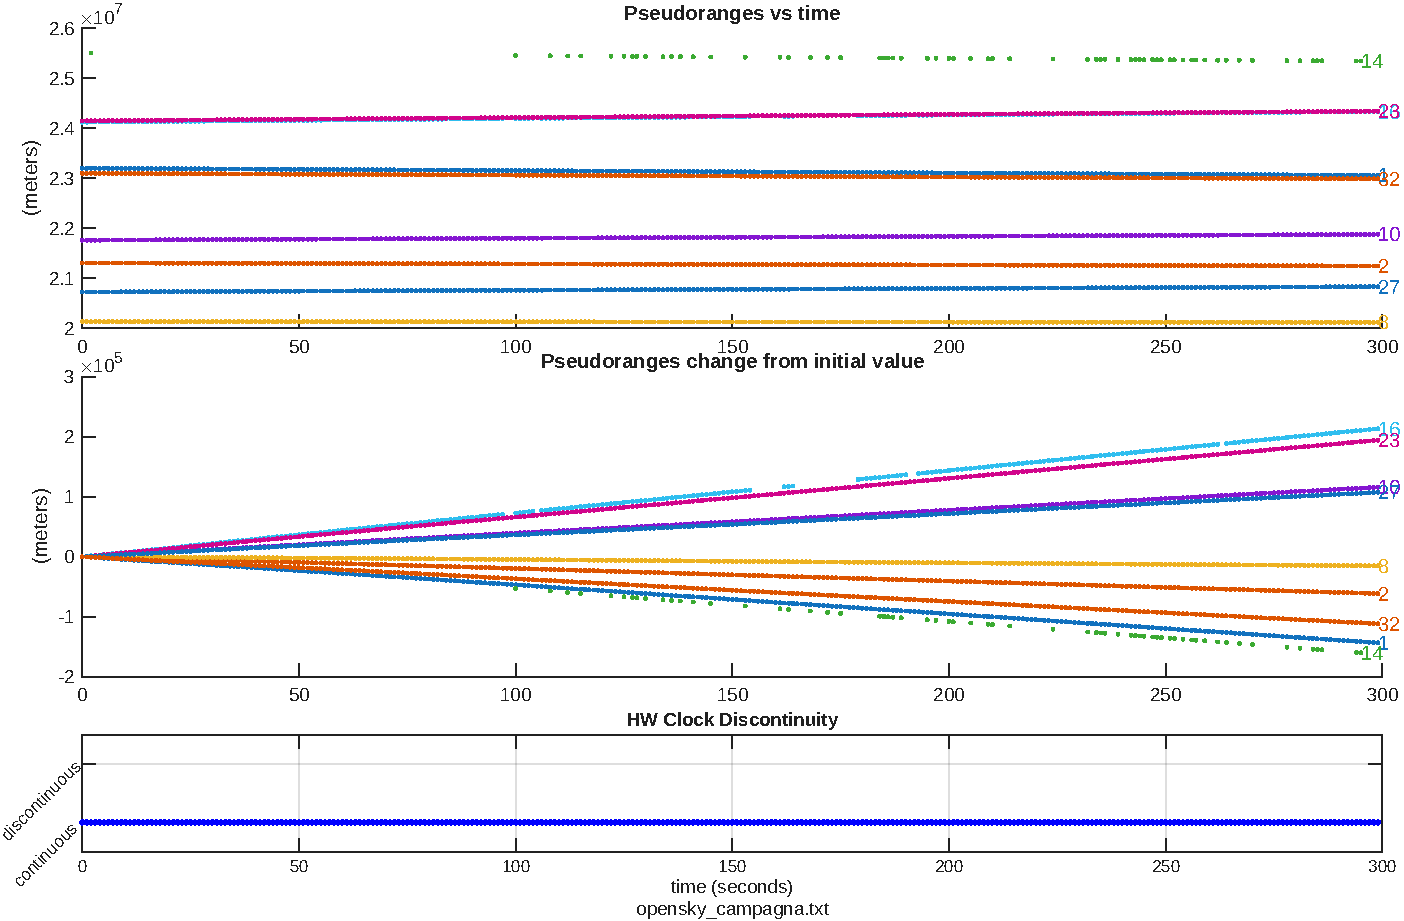
\includegraphics[width=\linewidth]{images/campagna_spoofing_no_delay/Figure_1.pdf}
      %  \caption{Pseudoranges evolution}
       % \label{fig:spoof_far_pr}
    %\end{subfigure}\hfill
    \begin{subfigure}{0.85\columnwidth}
        \centering
        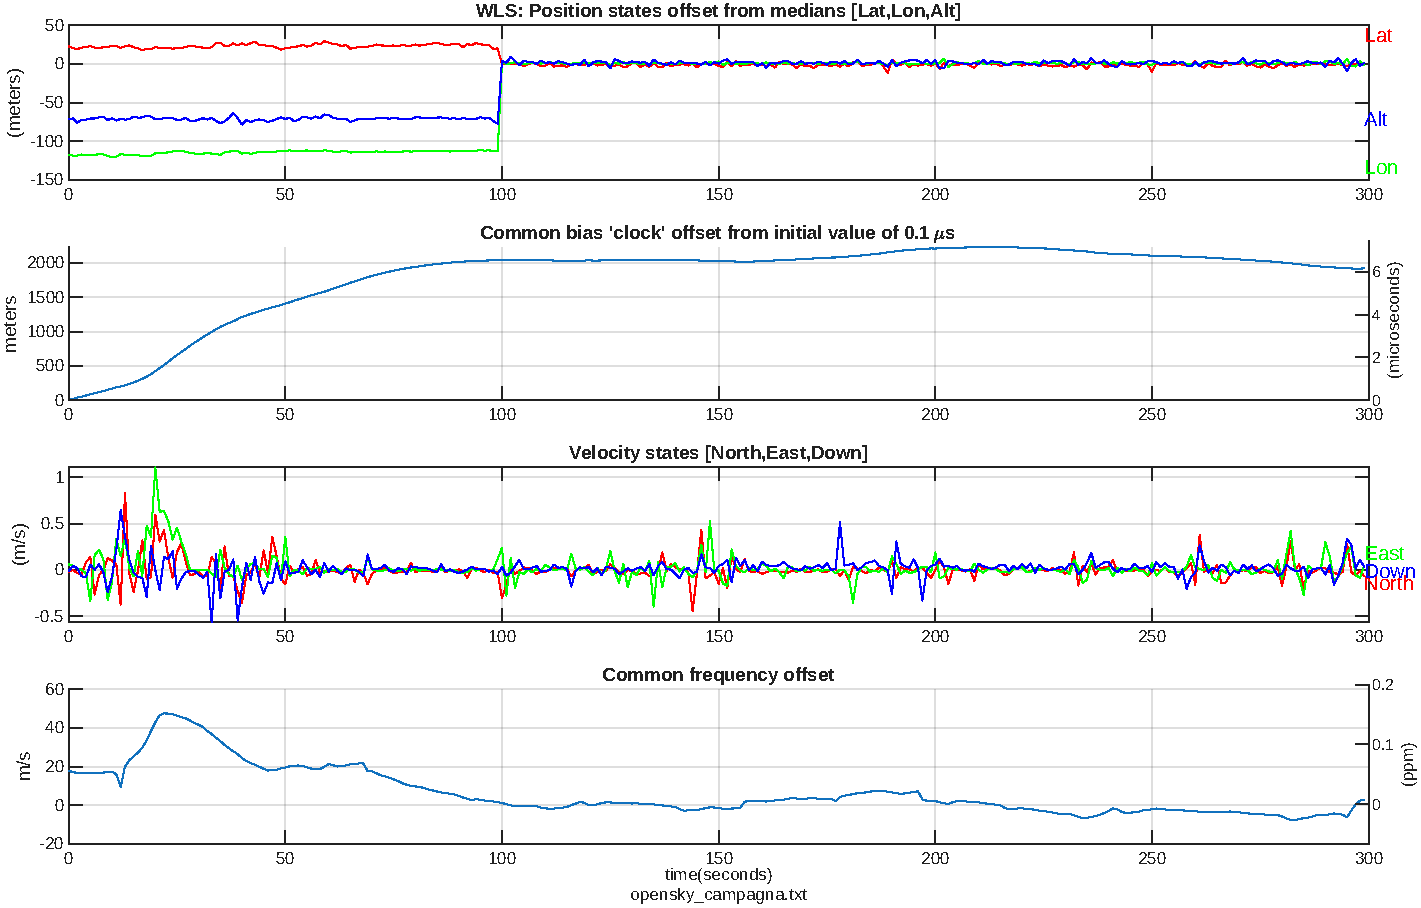
\includegraphics[width=\linewidth]{images/campagna_spoofing_no_delay/Figure_5.pdf}
        \caption{Position states and Clock bias}
        \label{fig:spoof_far_states}
    \end{subfigure}
    \label{fig:spoof_far_results}
\end{figure}

\subsection{Position Spoofing near receiver (with delay)}
In this second scenario, we injected both a false spatial position and a specific \texttt{spoof.delay} at 100 seconds: this new addition creates a massive vertical step across all pseudoranges simultaneously. Because satellite signals travel at the speed of light, even a fractional time delay introduced by the attacker translates into hundreds of kilometers of artificial distance added to every measurement. The WLS solver processes this new measurement and interprets it as a massive receiver clock error. As shown in Figure \ref{fig:spoof_delay_states}, while the spatial coordinates (latitude, longitude, altitude) still snap to the fake location, the clock bias experiences an instant, drastic jump exactly at 100 seconds. This behavior highlights a critical trade-off for an attacker: while introducing a delay might be physically necessary to "capture" the target receiver in a real-world over-the-air attack, it leaves an obvious anomaly in the clock bias domain.

\begin{figure}[htbp]
    \centering
    \begin{subfigure}{0.85\columnwidth}
        \centering
        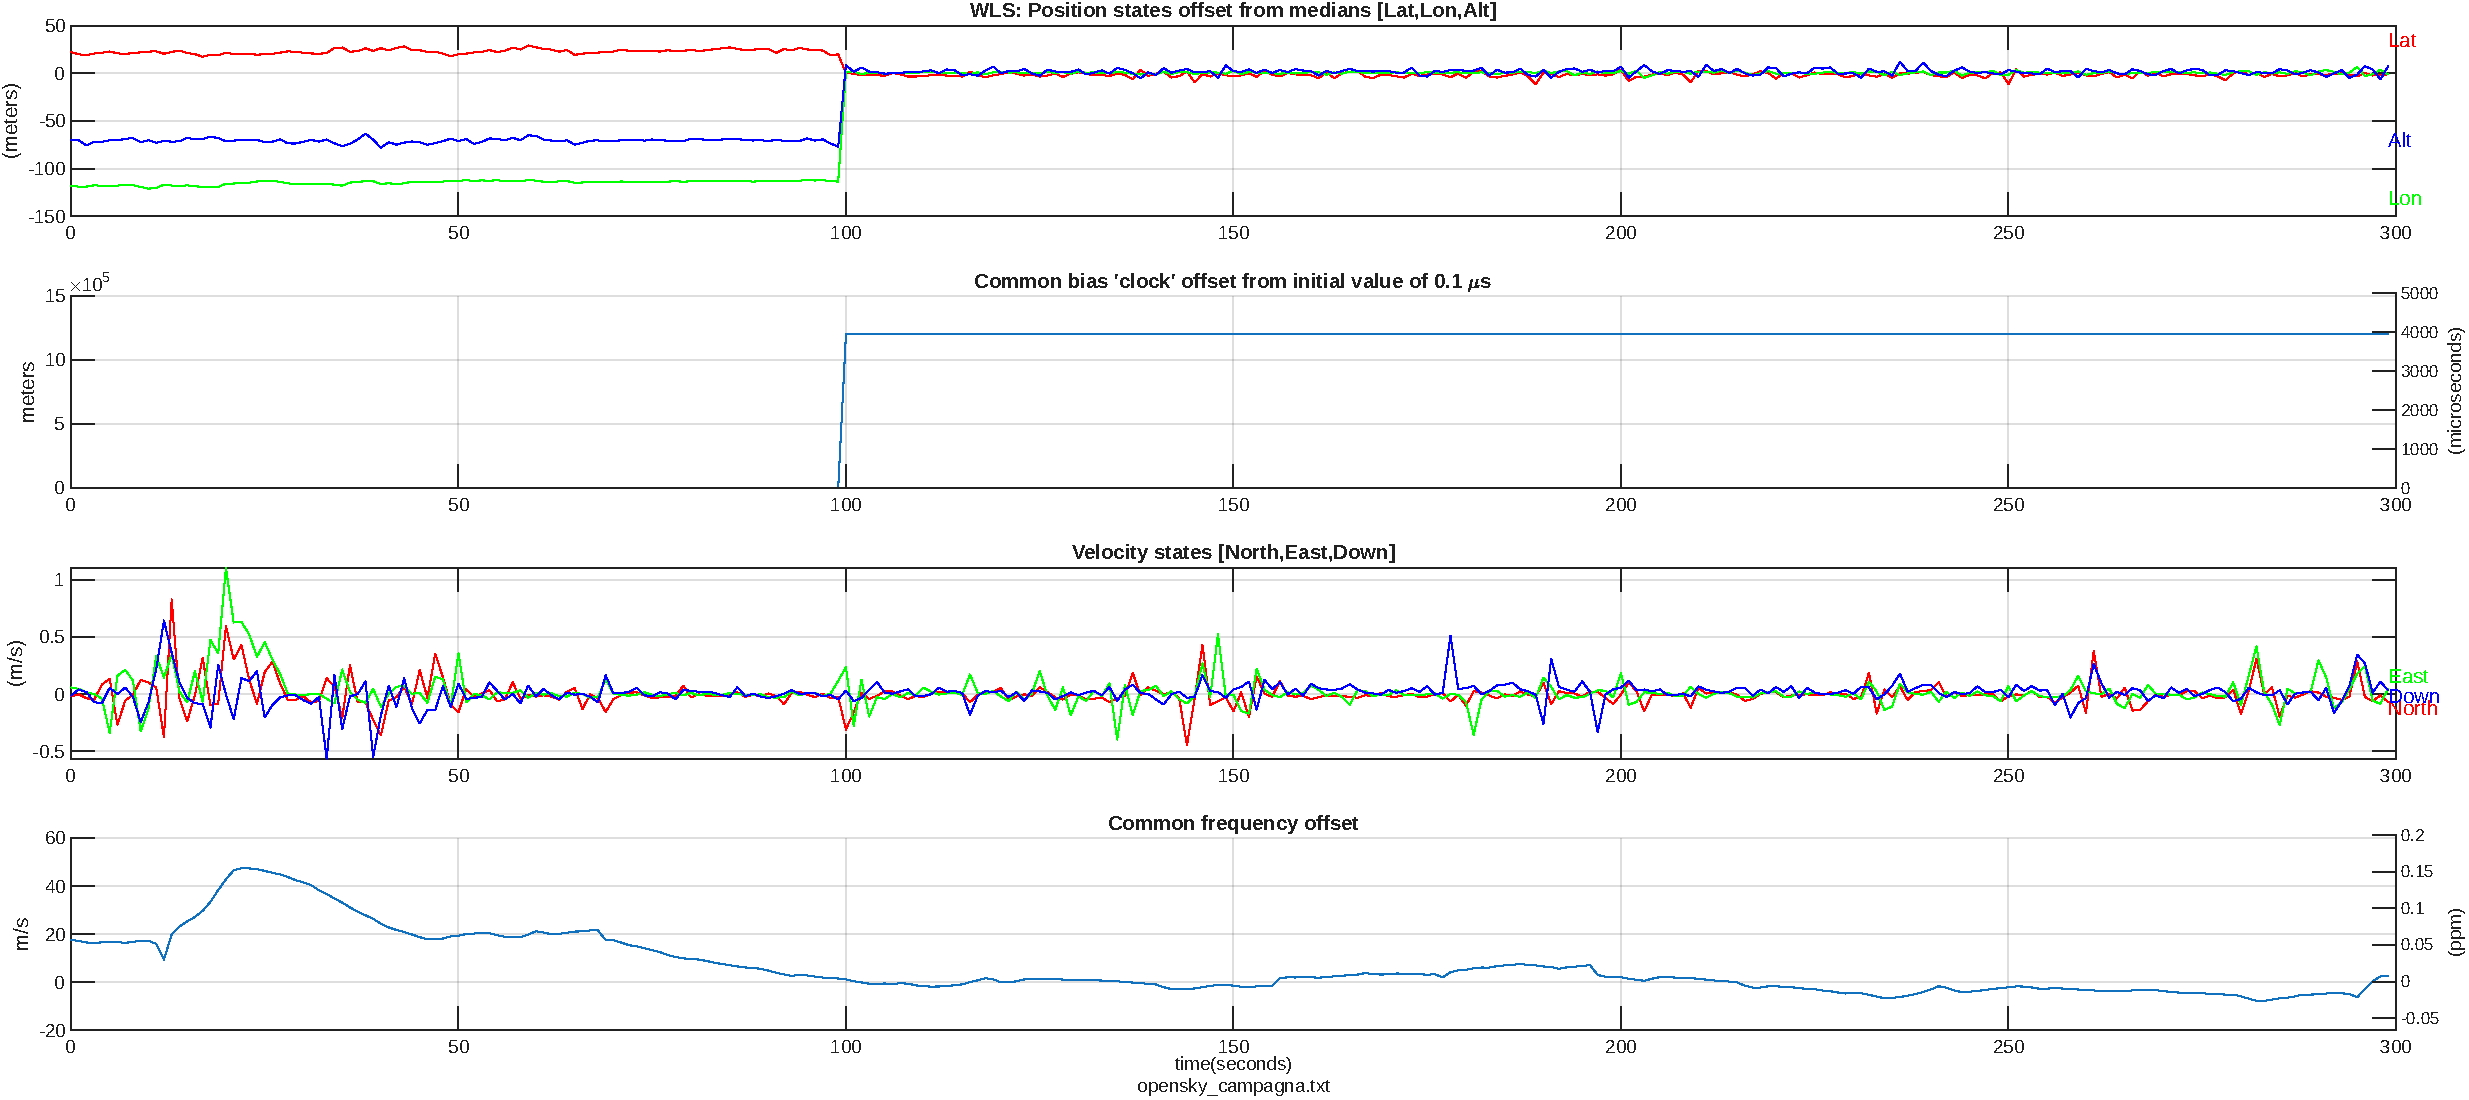
\includegraphics[width=\linewidth]{images/campagna_spoofing_delay/Figure_5.pdf}
        \caption{Position states and Clock bias jump}
        \label{fig:spoof_delay_states}
    \end{subfigure}
    \label{fig:spoof_delay_results}
\end{figure}


\subsection{Position Spoofing far from receiver (with delay)}

Here we executed a harsh spoofing experiment, shifting the target coordinates by approximately 478 km while simultaneously injecting a time delay. This attack represents a worst-case scenario where both the spatial and temporal domains are severely compromised. The "aggressive" spatial translation is evident in the WLS position states (Figure \ref{fig:spoof_torino_diff}): the offsets for latitude, longitude, and altitude immediately jump on the order of $10^5$ meters. Naturally, such an extreme discontinuity generates a completely unphysical and massive anomaly spike in the pseudorange rates. Consequently, the WLS solver is forced to compensate for this artificial propagation delay by forcefully adjusting the receiver's clock. As observed in the previous delayed scenario, the common bias clock violently spikes as shown in Figure \ref{fig:spoof_torino_states}. This specific test unequivocally demonstrates that while a "Far" spoofing attack can successfully teleport the computed position coordinates to a completely different geographic region, it leaves obvious traces across observed metrics.
\begin{figure}[htbp]
    \centering
    % Prima riga
    \begin{subfigure}{0.48\columnwidth}
        \centering
        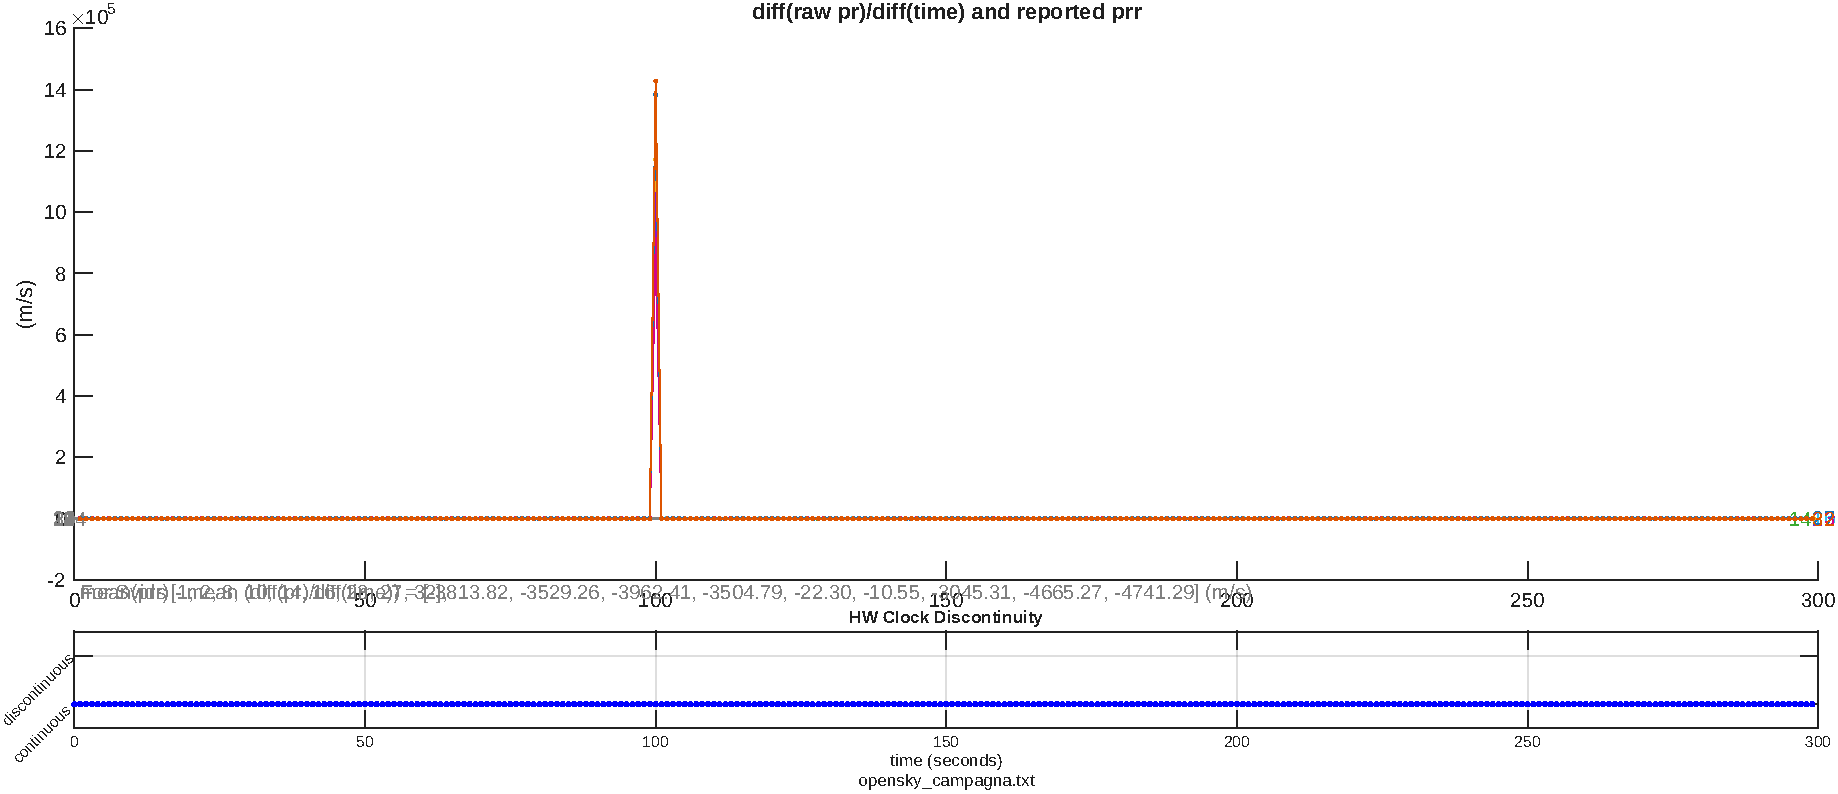
\includegraphics[width=\linewidth]{images/campagna_spoofing_delay_Torino/Figure_2.pdf}
        \caption{Pseudorange rates anomaly}
        \label{fig:spoof_torino_diff}
    \end{subfigure}\hfill
    \begin{subfigure}{0.48\columnwidth}
        \centering
        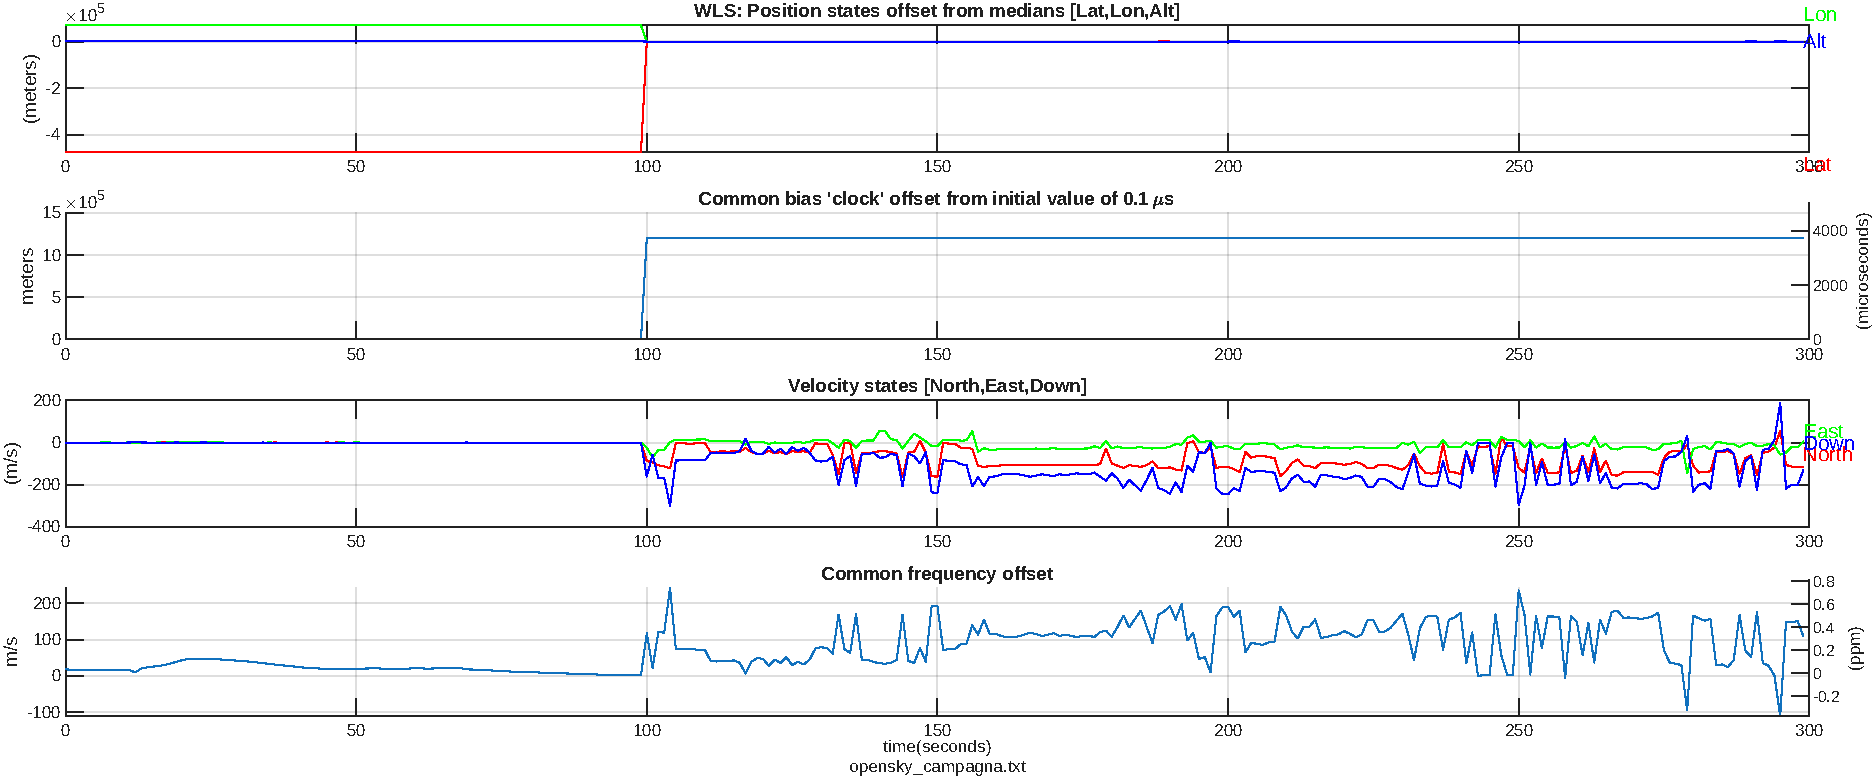
\includegraphics[width=\linewidth]{images/campagna_spoofing_delay_Torino/Figure_5.pdf}
        \caption{Position and Clock bias jump}
        \label{fig:spoof_torino_states}
    \end{subfigure}
\end{figure}


\subsection{Position Spoofing far from receiver (without delay)}

Lastly, we simulated another attack by forcing the coordinates similarly to the previous experiment but with the \texttt{spoof.delay} parameter disabled. The magnitude of the spatial jump forces the WLS solver to register again a violent discontinuity in the position states (Figure \ref{fig:spoof_torino_nodelay_states}), with offsets instantly surging by an order of $10^5$ meters and generating a massive spike in the pseudorange rates. But the most revealing metric here is the receiver's internal clock: since no artificial time delay was introduced, the common bias clock smoothly follows its natural continuous drift. This physical behavior confirms that the WLS solver interpreted the manipulated measurements strictly as an instantaneous spatial teleportation, compromising the position domain while leaving the temporal synchronization intact.
\begin{figure}[htbp]
    \centering
    \begin{subfigure}{0.48\columnwidth}
        \centering
        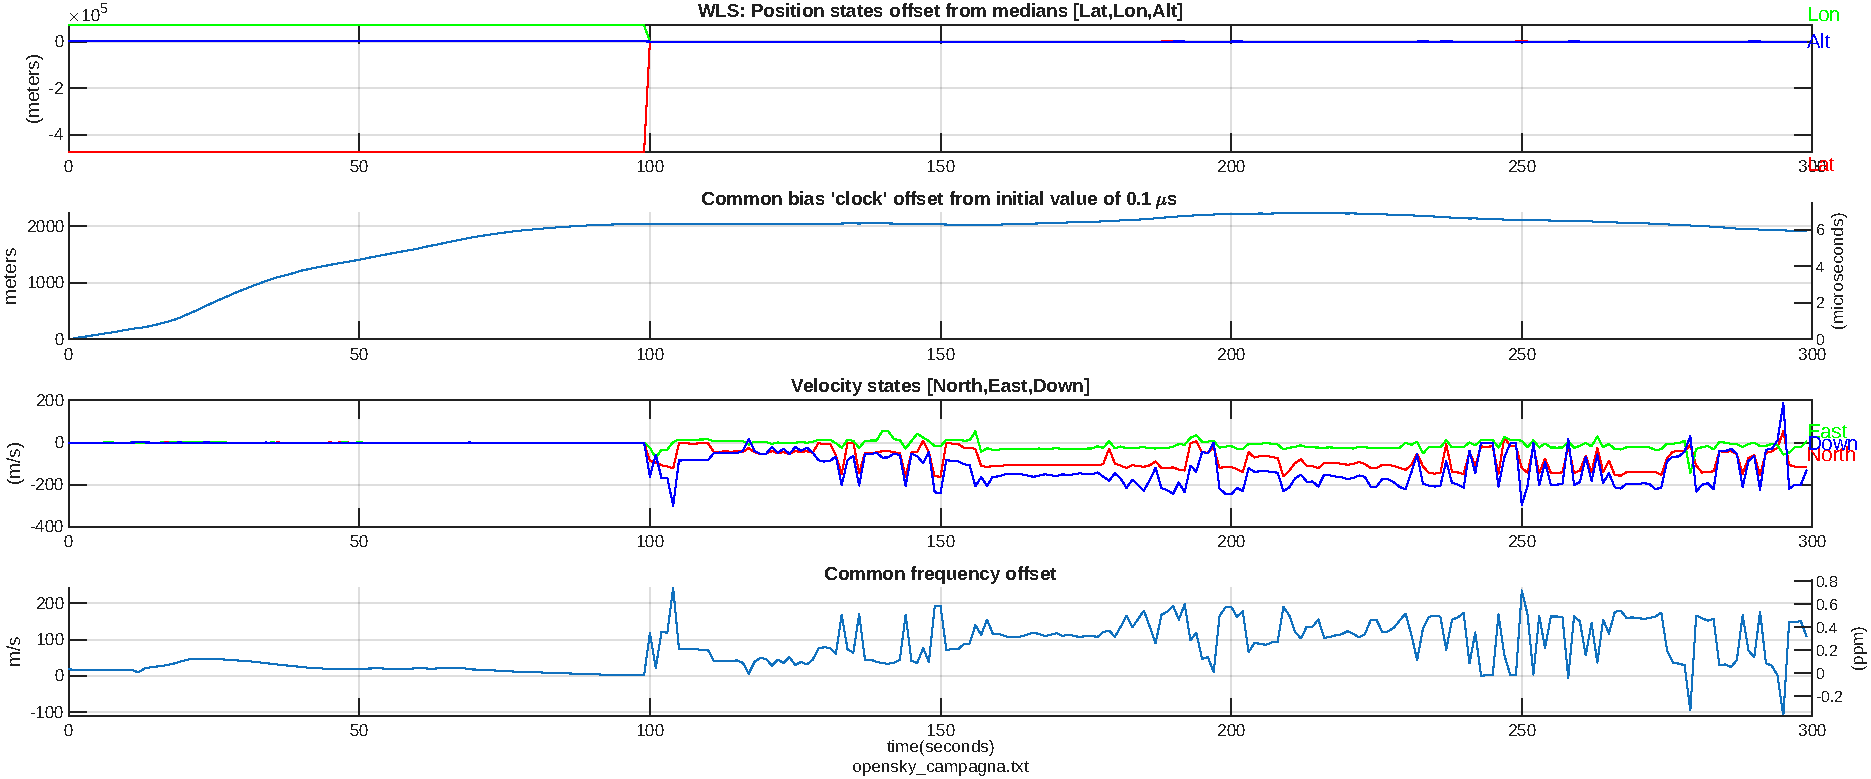
\includegraphics[width=\linewidth]{images/campagna_spoofing_no_delay_Torino/Figure_5.pdf}
        \caption{Position jump of $\times 10^5$ m with continuous clock}
        \label{fig:spoof_torino_nodelay_states}
    \end{subfigure}
    \begin{subfigure}{0.48\columnwidth}
        \centering
        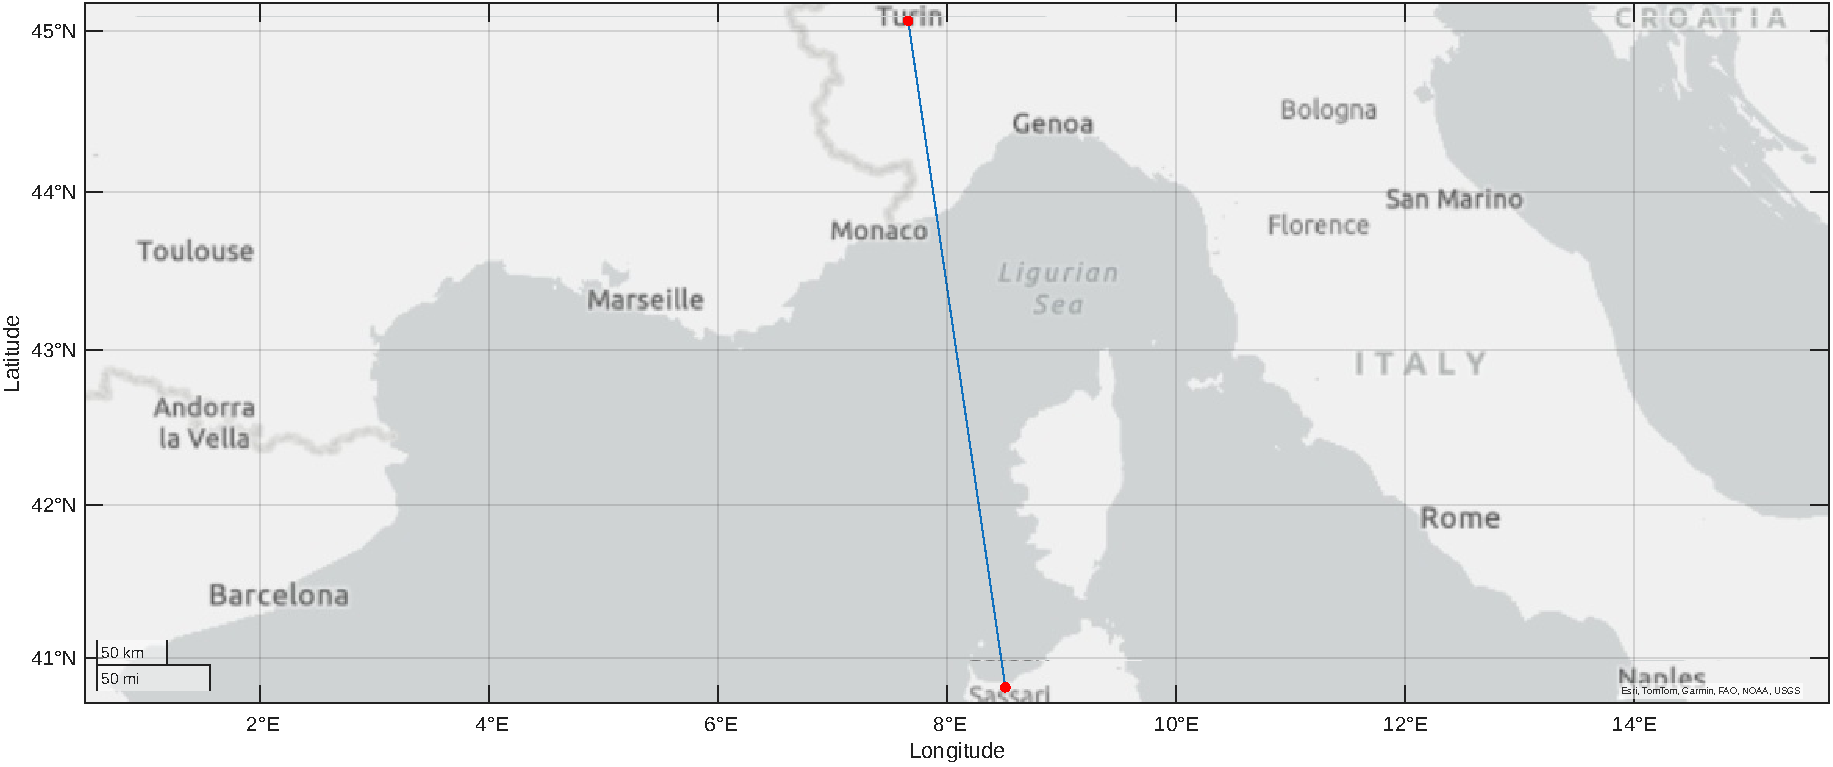
\includegraphics[width=\linewidth]{images/campagna_spoofing_no_delay_Torino/[Optional] Plot Positioning Solution on Map.pdf}
        \caption{Actual location vs physical position}
        \label{fig:spoof_torino_nodelay_position}
    \end{subfigure}
    \label{fig:spoof_torino_nodelay_results}
\end{figure}
\section{Measurements}
\label{sec:Measurements}

\subsection{Open sky}
This is the ideal setting, where the receiver is not moving and the satellites are in line-of-sight, ensuring optimal signal reception. The 50\% position distribution has a 1.9 m radius (Figure \ref{fig:campagna_pvt_hdop}) and the number of satellites remains around 7 to 9 throughout the measurement.
The horizontal speed variation is at most around 1.30 m/s (the device was slightly moved during the start of the measurement) and the HDOP, which measures how the
satellite geometry affects the accuracy of the horizontal position, remains
mostly stable at 1 or lower, spiking only when the satellites drop to 7.

\begin{figure}[H]
    \centering
    \begin{subfigure}{0.80\columnwidth}
        \centering
        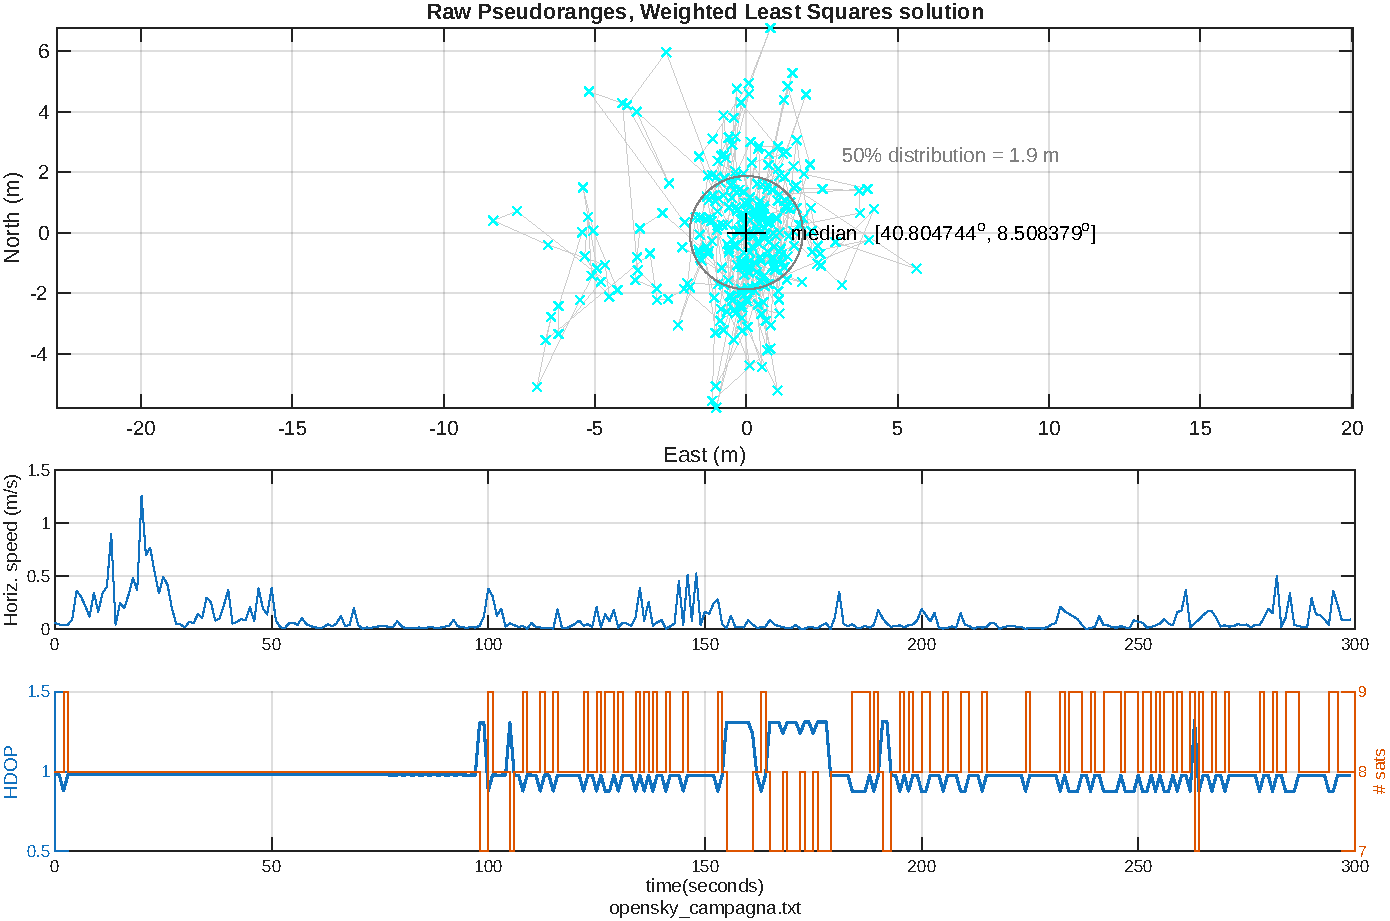
\includegraphics[width=\linewidth]{images/opensky_campagna/Figure_4.pdf}
        \caption{Position estimate, Horizontal speed and HDOP}
        \label{fig:campagna_pvt_hdop}
    \end{subfigure}
    
    % RIGA VUOTA FONDAMENTALE PER ANDARE A CAPO
    \vspace{0.5cm} % Spazio per distanziare le due figure
    
    \begin{subfigure}{0.80\columnwidth}
        \centering
        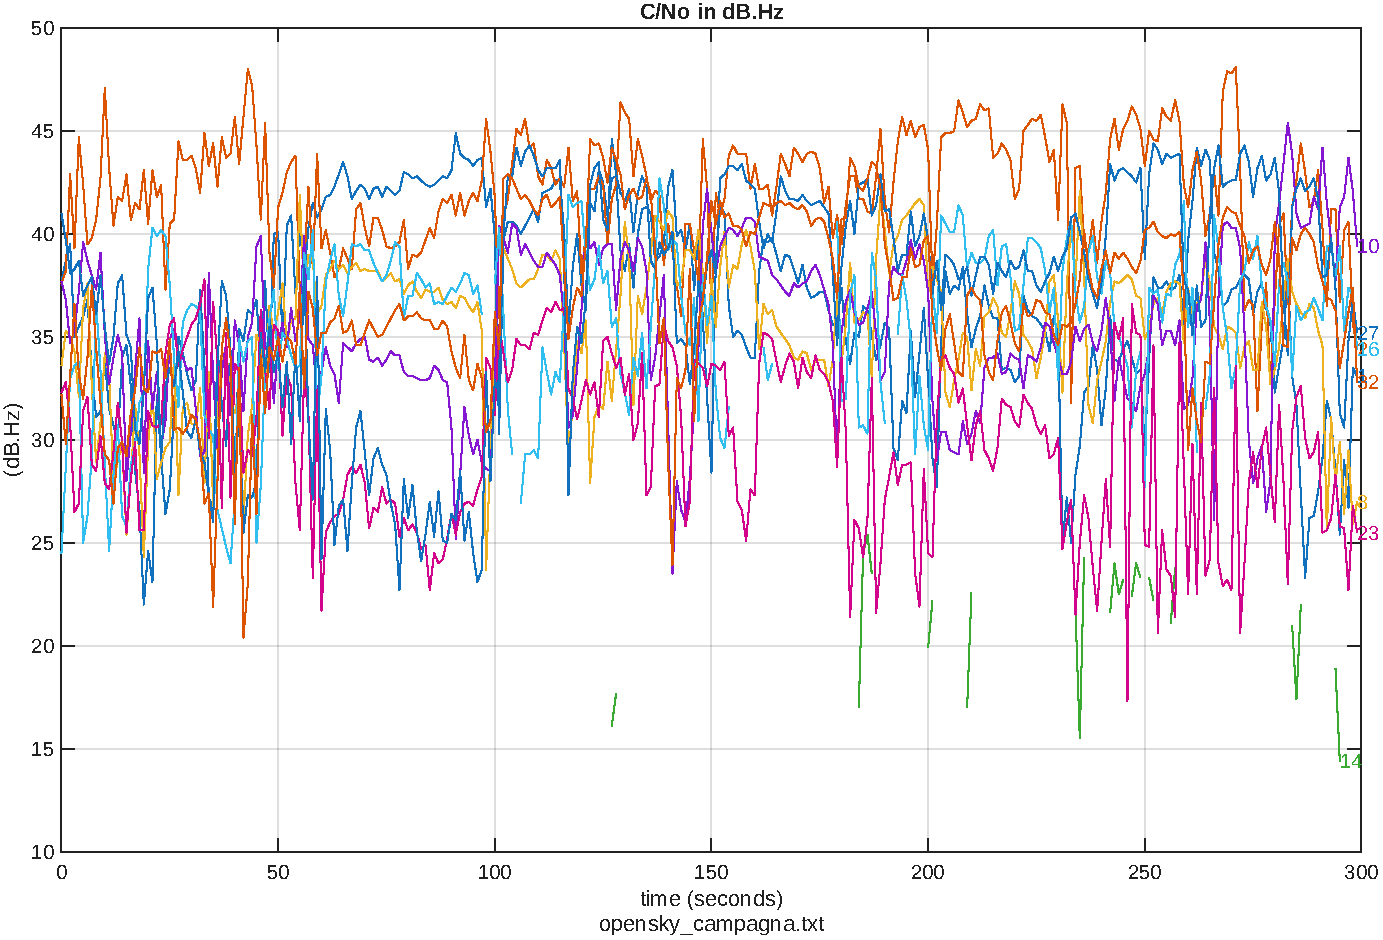
\includegraphics[width=\linewidth]{images/opensky_campagna/Figure_3.pdf}
        \caption{C/N0}
        \label{fig:opensky_cn0}
    \end{subfigure}
    
    \label{fig:opensky_results}
\end{figure}

\subsection{Outdoor walking}
Here, the horizontal speed fluctuates mostly between 0.5 and 2.0 m/s, which is consistent with normal walking. The 4.3 m/s velocity spikes are not possible for a pedestrian, confirming multipath interference at certain intersections and resulting in positioning "jumps". Satellite geometry exhibits noticeable vulnerability: while HDOP is mostly around 0.9-1.0, it sharply peaks at 1.8 when the number of tracked satellites temporarily drops to its minimum of 6 (Figure \ref{fig:walking_cno}). The C/N0 plot also confirms the dynamic conditions; while the strongest signals occasionally peak at 40-41 dB-Hz, several satellites experience deep fading, plunging below 15 dB-Hz (e.g., SVID 11 and 32). These frequent signal drops are direct evidence of severe line-of-sight obstructions along the walking path.

\begin{figure}[H]
    \centering
    \begin{subfigure}{0.85\columnwidth}
        \centering
        % ATTENZIONE: qui hai usato lo stesso nome file (Figure_4_1.pdf). 
        % Modificalo se la seconda immagine ha un nome diverso (es. Figure_4_2.pdf)!
        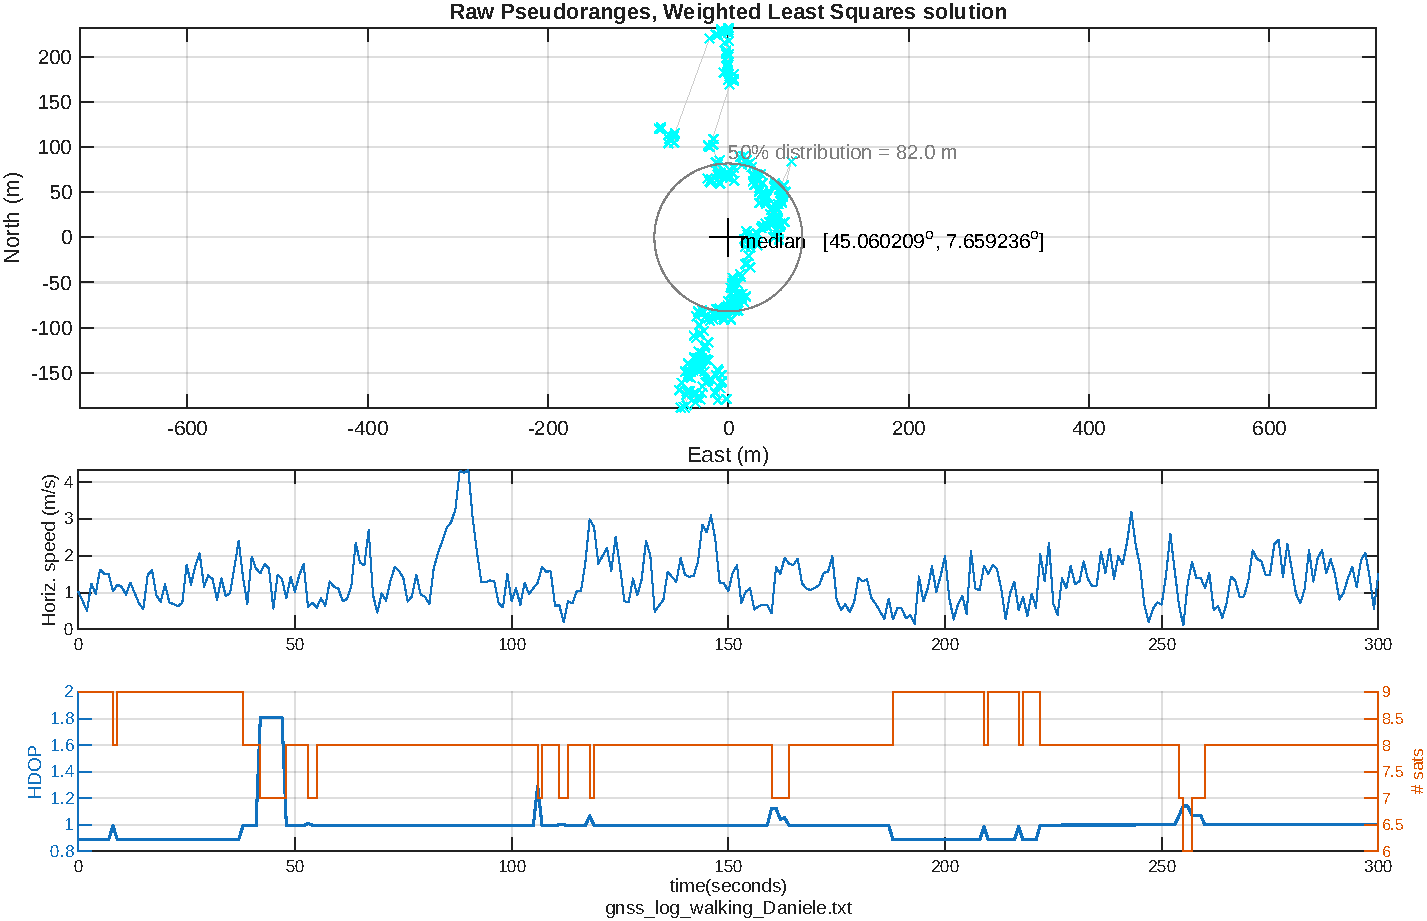
\includegraphics[width=\linewidth]{images/walking_Daniele/Figure_4.pdf}
        \label{fig:walking_sp_hdop}
    \end{subfigure}
    
    %\vspace{0.5cm} % Aggiunge un piccolo spazio verticale tra la prima e la seconda riga
    
    % Seconda riga: terza immagine centrata in basso
    \begin{subfigure}{0.85\columnwidth}
        \centering
        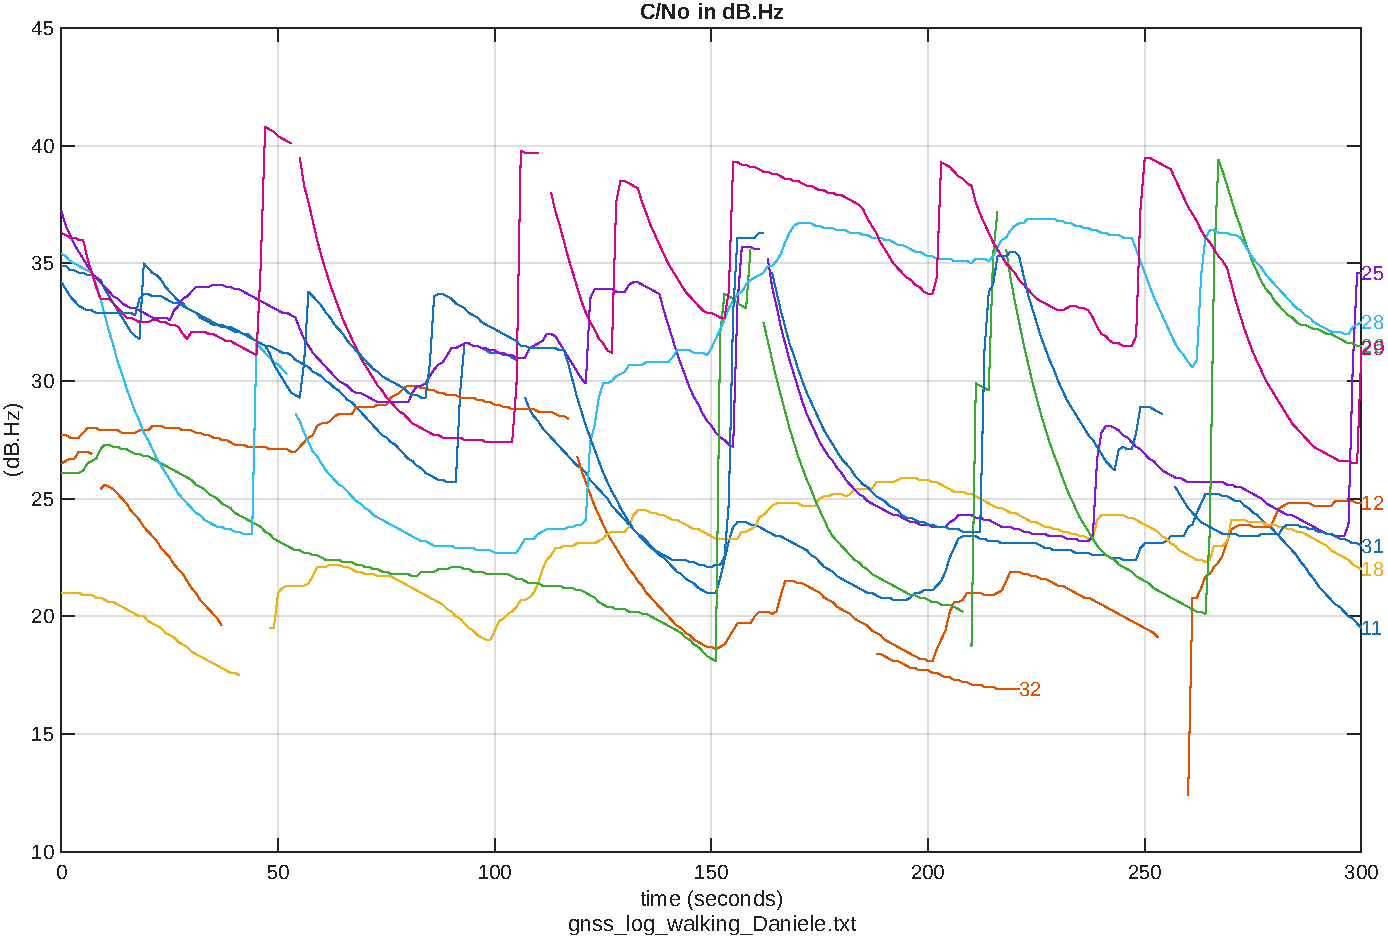
\includegraphics[width=\linewidth]{images/walking_Daniele/Figure_3.pdf}
        \caption{Horizontal speed, HDOP and Carrier over Noise}
        \label{fig:walking_cno}
    \end{subfigure}
    \label{fig:walking_results}
\end{figure}

\subsection{Outdoor Bus}
For this measurement, the receiver is located inside a moving bus, so the line of sight is partially obstructed. Figure \ref{fig:bus_results} shows the receiver’s velocity with peaks around 14 m/s (around 50 km/h), which makes sense since the log was registered inside an urban area. The number of visible satellites ranges from 7 to 11 with the corresponding HDOP spikes, probably due to many obstacles around, such as buildings obstructing the line of sight during the trip.

\begin{figure}[H]
    \begin{subfigure}{0.85\columnwidth}
        \centering
        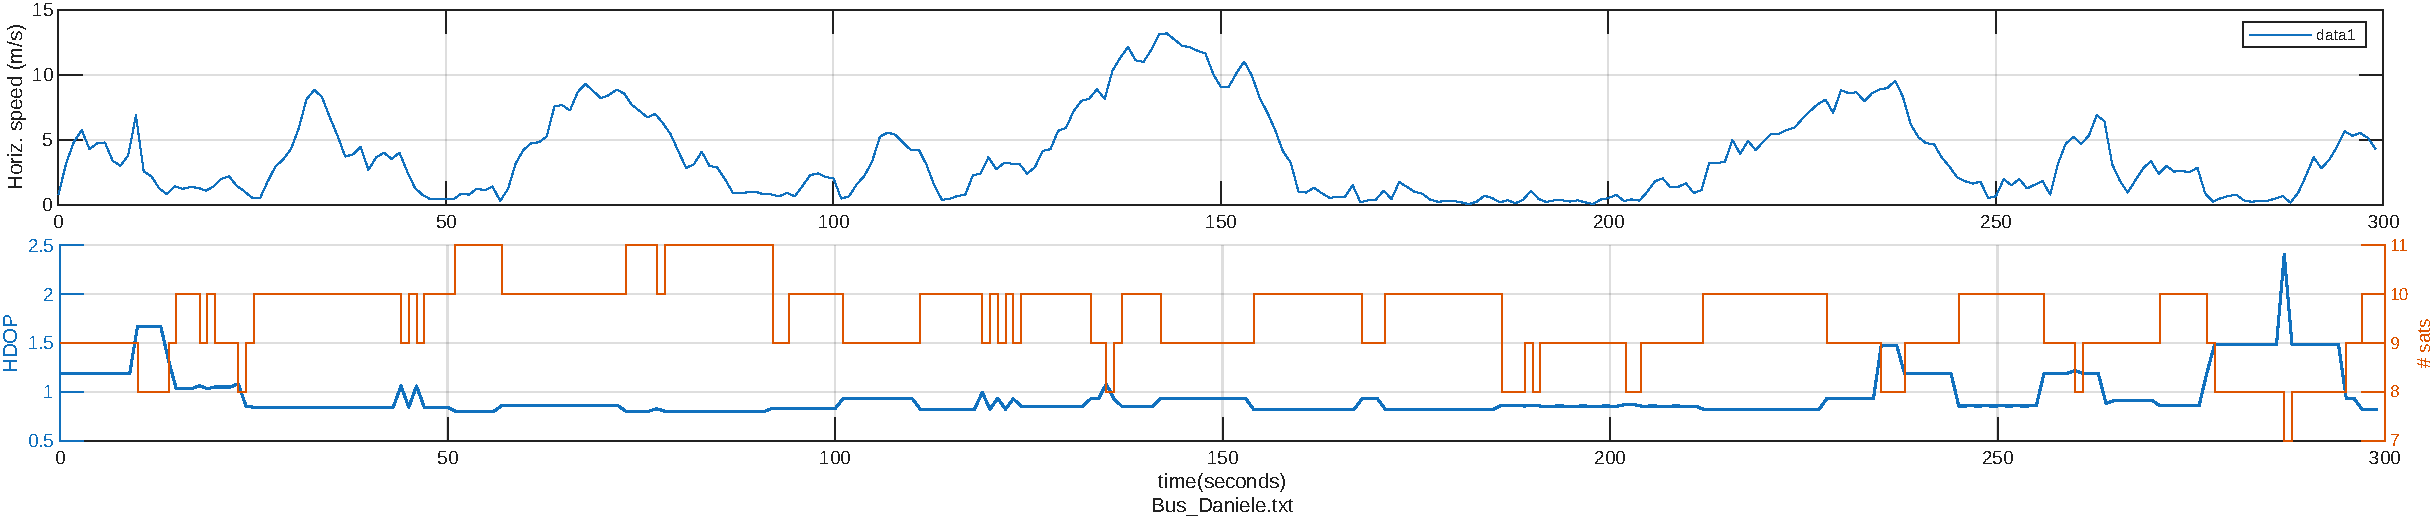
\includegraphics[width=\linewidth]{images/Bus_Daniele/Figure_4.pdf}
        \caption{Horizontal speed and HDOP}
        \label{fig:bus_hdop}
    \end{subfigure}
    \begin{subfigure}{0.85\columnwidth}
        \centering
        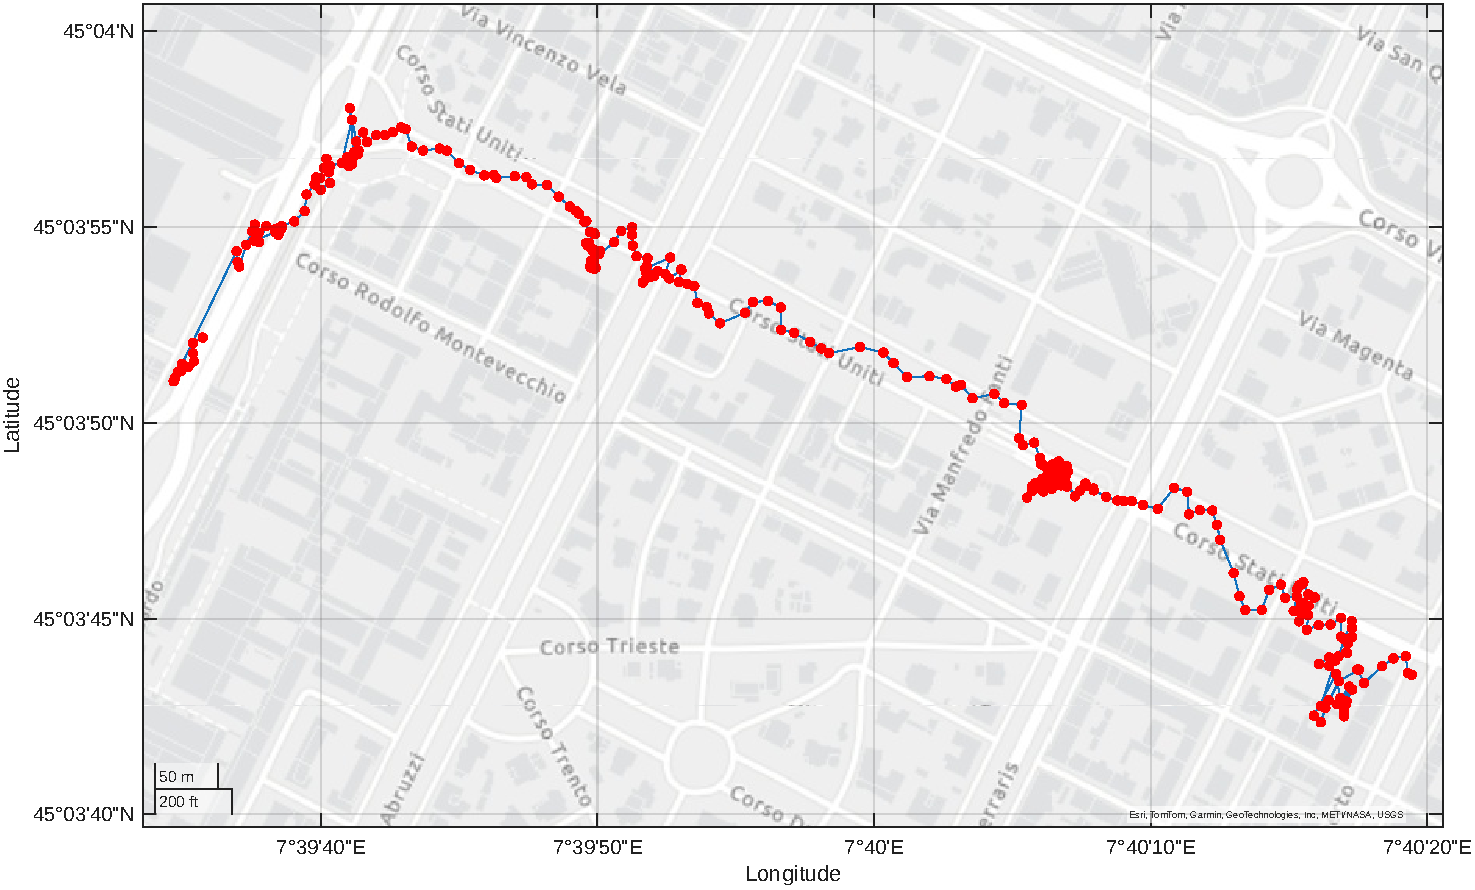
\includegraphics[width=\linewidth]{images/Bus_Daniele/[Optional] Plot Positioning Solution on Map.pdf}
        
        \label{fig:bus_map}
    \end{subfigure}
    \caption{Horizontal speed, HDOP and movement map}
    \label{fig:bus_results}
\end{figure}

\subsection{Body interference}
The aim of this measurement is to analyze the impact of signal obstruction caused by the human body. This happens because our body absorbs radio waves in the GNSS L-bands, acting as an attenuating shield that obstructs signal reception. The 5-minute recording is divided into two parts: in the first 2 minutes the receiver is in normal conditions, and in the next 3 minutes the device is on the chest of the operator, covered by his hands. The first indicator of the scenario change is the C/N0 graph (Figure \ref{fig:body_cno}) where levels during the initial 120 seconds are steady and comparatively high (35/45 dB-Hz), indicative of clean reception. The strength of the signals drops to about 10-15 dB-Hz when the phone is placed near the chest: this interference is clearly visible in the three panels of Figure \ref{fig:body_pvt_hdop}, where the number of satellites (orange line) after 120 seconds becomes unstable along with tracking losses. As a result, the HDOP (blue line) increases and reaches a peak. When some satellites are lost, the geometry of the visible constellation is compromised, resulting in deterioration of accurate positioning. Although the receiver remained stationary throughout the test, the velocity plot shows significant noise after 120 seconds, almost certainly due to low C/N0 and multipath induced by body proximity. In the scatter plot, the dispersion of the points increases consistently in the second phase: while the first points are concentrated near the origin, the next ones suggest systematic errors resulting from interference.

\begin{figure}[htbp]
    \centering
    % Prima riga: C/N0 (Figure 3)
    \begin{subfigure}{0.85\columnwidth}
        \centering
        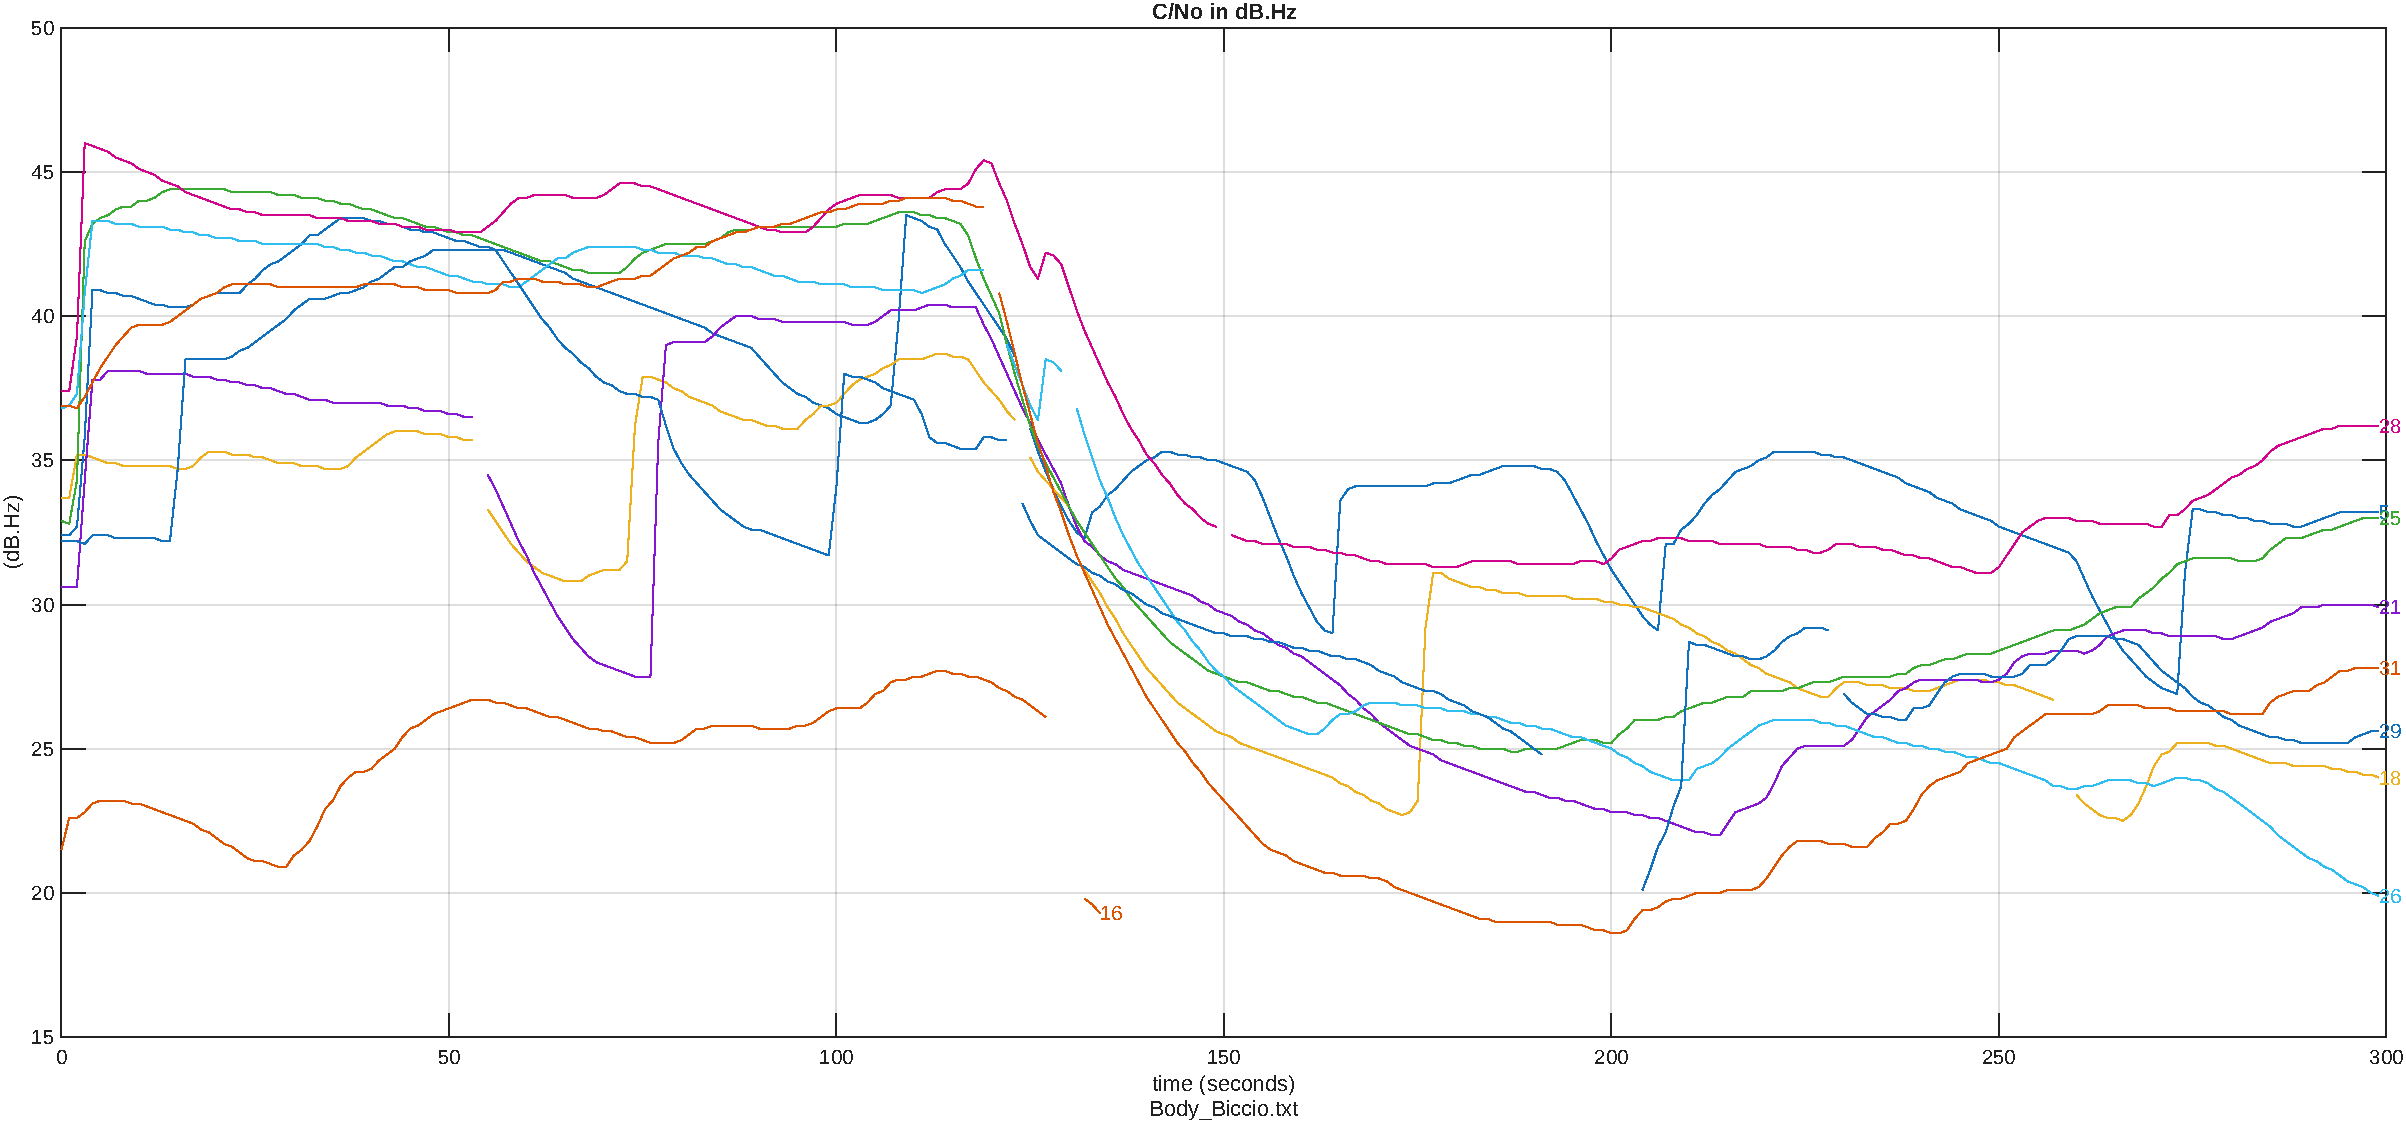
\includegraphics[width=\linewidth]{images/Body_Biccio/Figure_3.pdf}
        \caption{C/N0 in dB.Hz }
        \label{fig:body_cno}
    \end{subfigure}
    
    \vspace{0.4cm} % Spazio verticale tra le righe
    
    % Seconda riga: Speed, HDOP e Position (Figure 4)
    \begin{subfigure}{0.85\columnwidth}
        \centering
        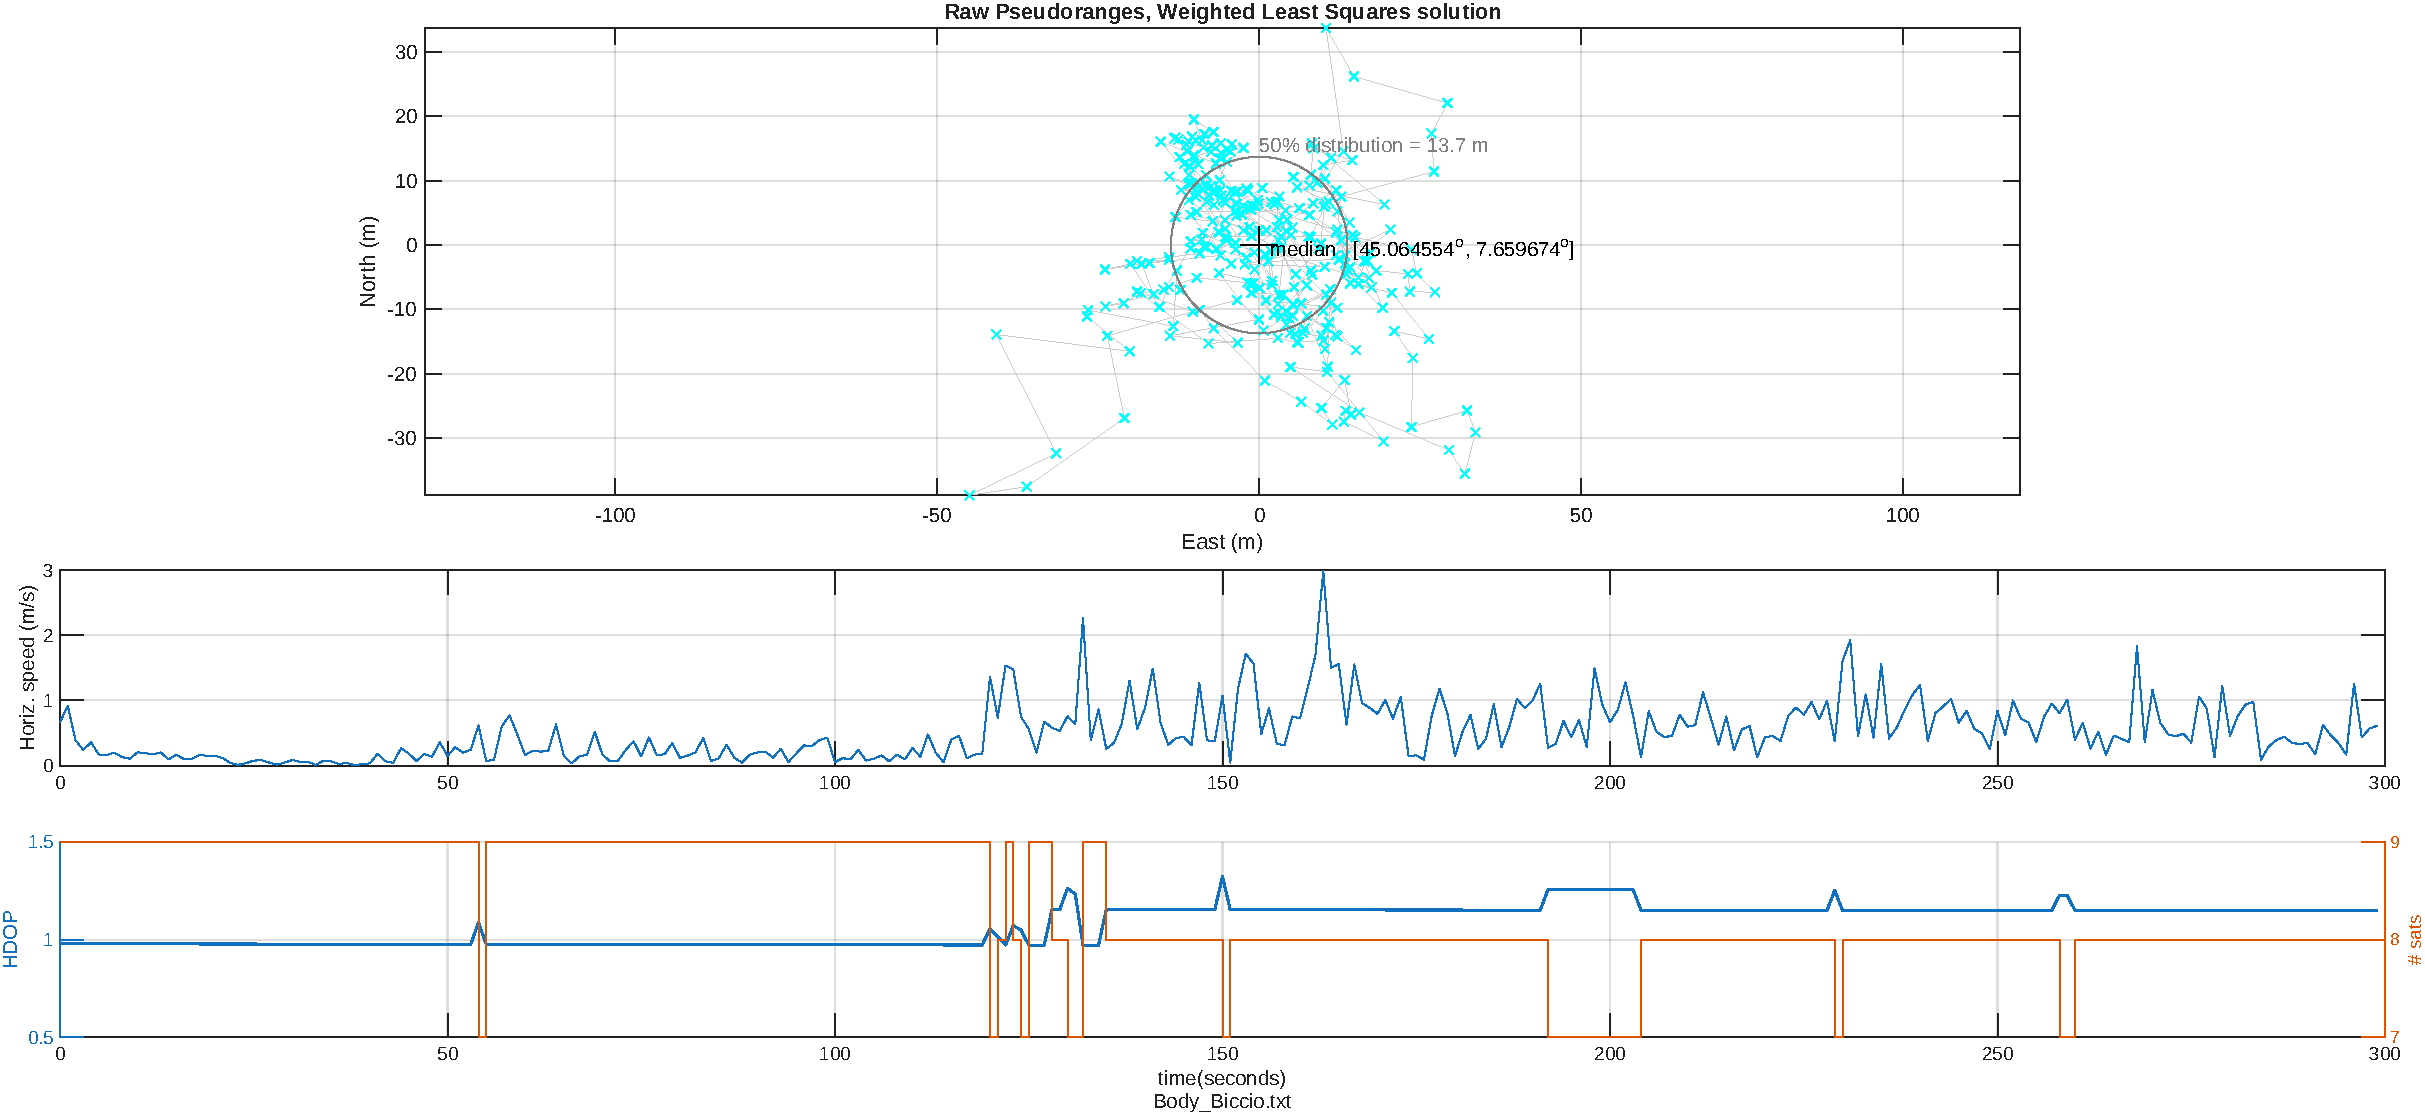
\includegraphics[width=\linewidth]{images/Body_Biccio/Figure_4.pdf}
        \caption{Position estimate, Horizontal speed and HDOP}
        \label{fig:body_pvt_hdop}
    \end{subfigure}
    \vspace{0.3cm} % Spazio verticale tra le righe
    \label{fig:body_results}
\end{figure}

























\subsection{Aluminum Interference}
    In this experiment, we simulated a Faraday cage using a sheet of aluminum foil, leaving a small opening to allow a portion of the satellite signals to pass through. The $C/N_0$ analysis in Figure \ref{fig:cno_stagnola} confirms that placing our smartphone inside an aluminum foil caused an immediate and severe attenuation of the signals.
    Satellites 4 and 11 disappeared, and other signals' power decreased significantly with levels between 20 and 35 dB-Hz. On the other hand, signals from satellites 5 to 29 showed relative stability or intermittent peaks, proving that these satellites were periodically aligned with the uncovered portion of the foil. The signal instability is clearly visible in Figure \ref{fig:graph_stagnola_pseudo} but the clock remained stable. 
    \noindent Figure \ref{fig:hdop_stagnola} reveals a significant spread of data points, characterized by a 50\% distribution error of 18.0 meters from the median position. Even though the smartphone was fixed in place, the horizontal speed graph displays anomalous velocity peaks, reaching up to 10 m/s due to phase noise and multipath reflections caused by the metal foil. This instability is also reflected in the satellite geometry, as the HDOP value lies between 1.5 and 2.5 due to satellites frequently being lost and reacquired through the hole. The experiment demonstrates that even partial shielding is enough to compromise positioning accuracy, even though hardware clock continuity was maintained throughout the test.
    
    \begin{figure}[H]
        \centering
        % Prima riga: due immagini affiancate
        \begin{subfigure}{0.48\columnwidth}
            \centering
            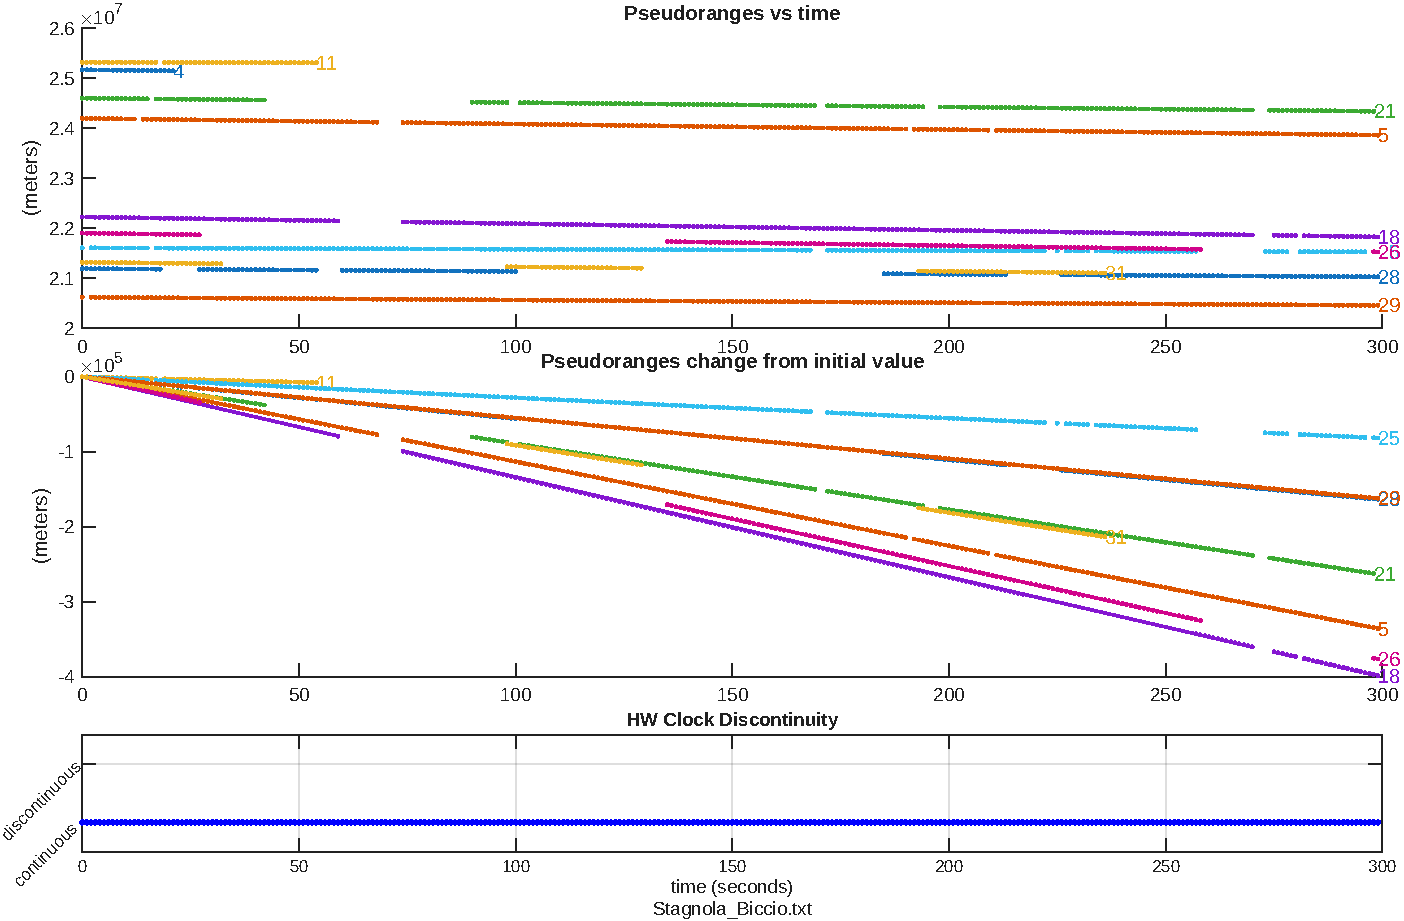
\includegraphics[width=\linewidth]{images/Stagnola_Biccio/Figure_1.pdf}
            \caption{Pseudorange \& HW Clock }
            \label{fig:graph_stagnola_pseudo}
        \end{subfigure}\hfill
        \begin{subfigure}{0.48\columnwidth}
            \centering
            % ATTENZIONE: qui hai usato lo stesso nome file (Figure_4_1.pdf). 
            % Modificalo se la seconda immagine ha un nome diverso (es. Figure_4_2.pdf)!
            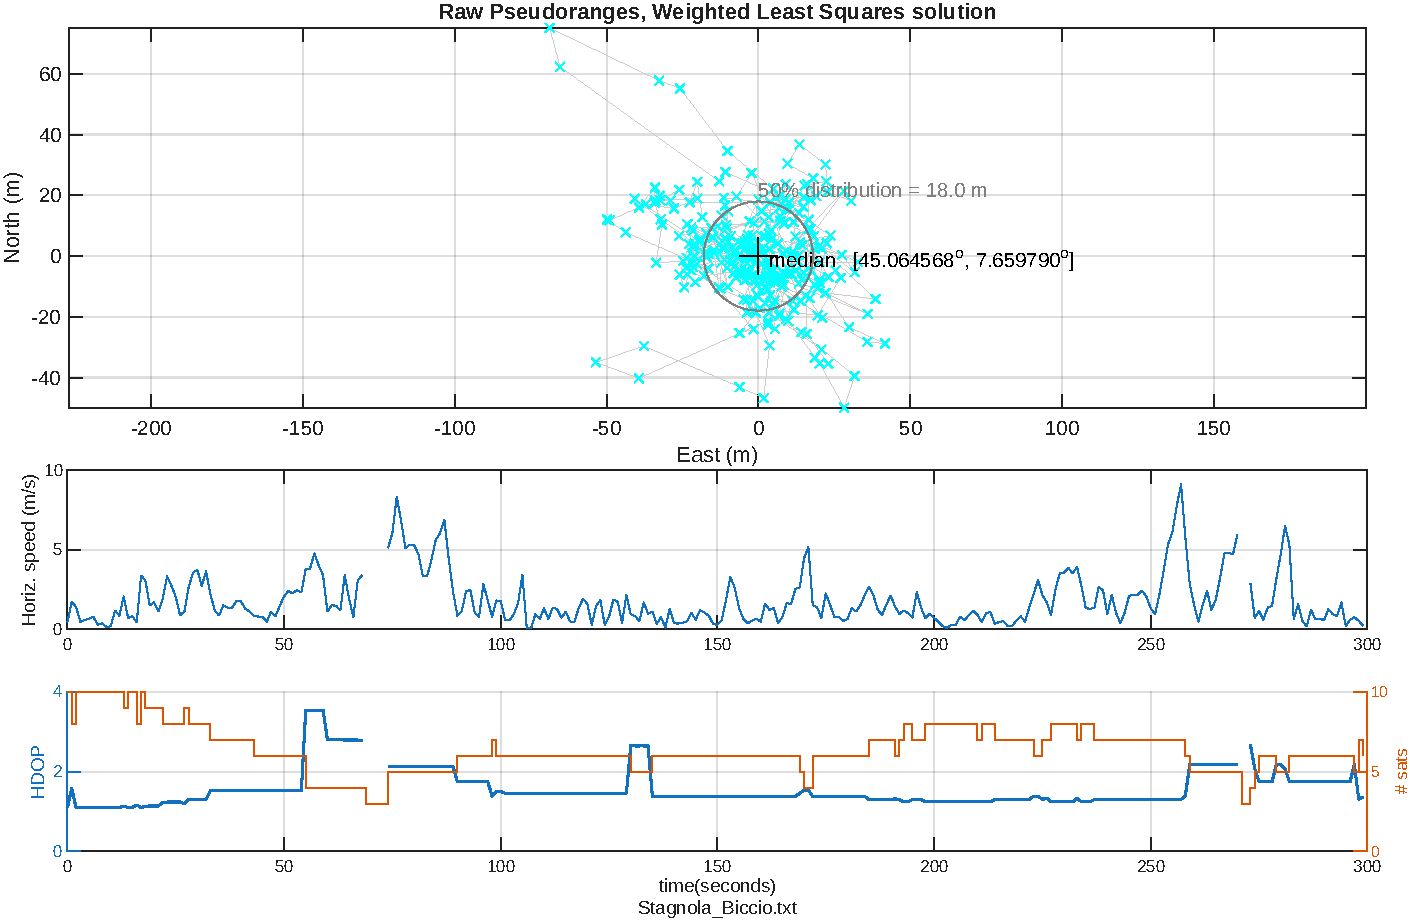
\includegraphics[width=\linewidth]{images/Stagnola_Biccio/Figure_4.pdf}
            \caption{Position Error, HDOP \& N. Sat}
            \label{fig:hdop_stagnola}
        \end{subfigure}
        
        \vspace{0.4cm} % Aggiunge un piccolo spazio verticale tra la prima e la seconda riga
        
        % Seconda riga: terza immagine centrata in basso
        \begin{subfigure}{0.85\columnwidth}
            \centering
            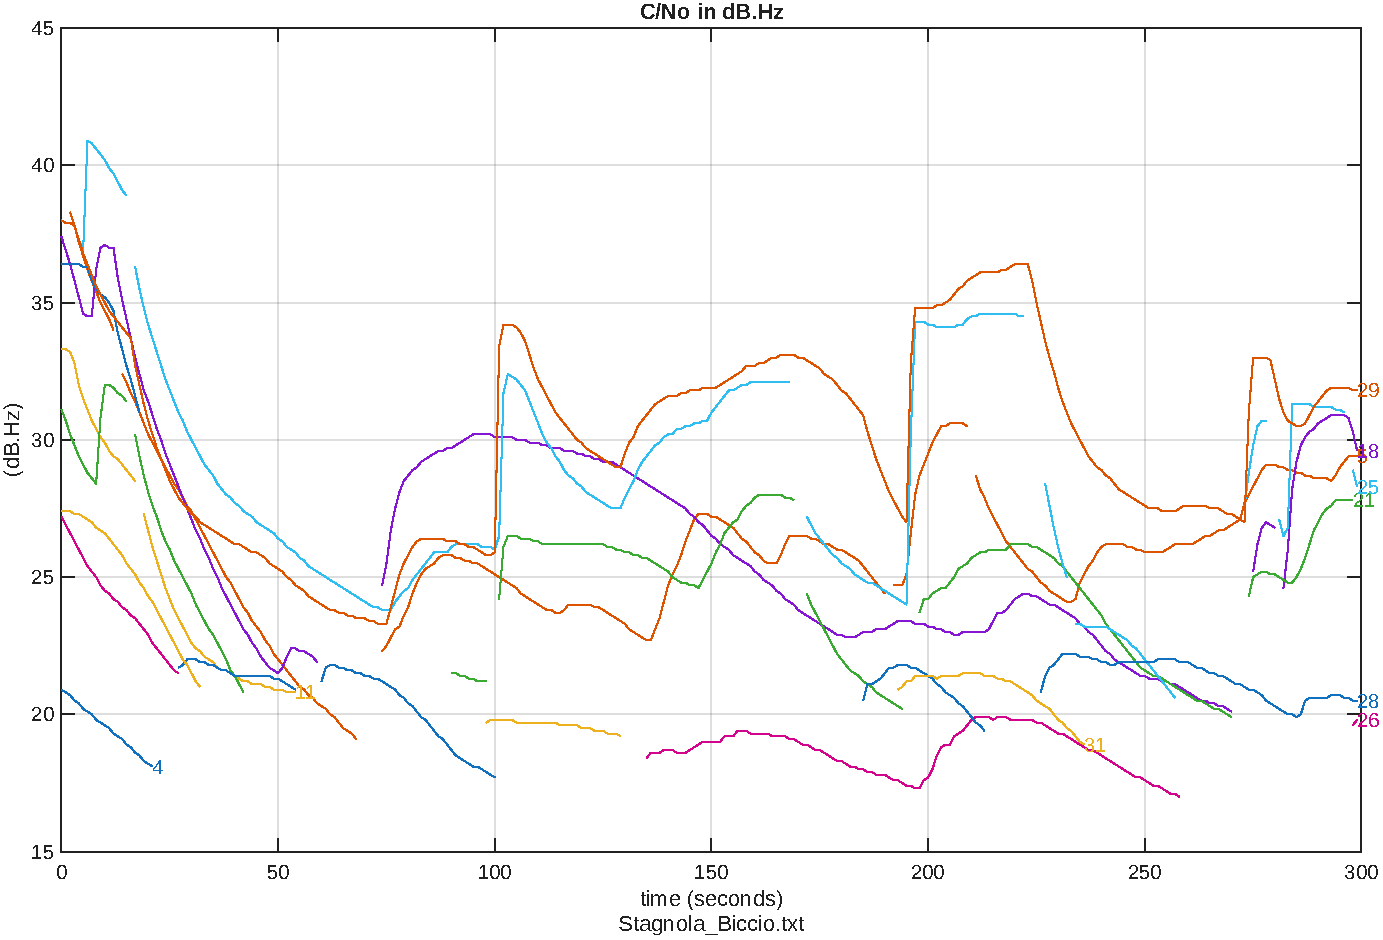
\includegraphics[width=\linewidth]{images/Stagnola_Biccio/Figure_3.pdf}
            \caption{C/N0}
            \label{fig:cno_stagnola}
        \end{subfigure}
        \label{fig:aluminium_results}
    \end{figure}
    


%\vspace{0.4cm}


\section{Spoofing}
This section will explore the impact of simulated cyber-spoofing attacks, which were performed by manipulating the previously captured open sky measurement. We triggered different attack conditions starting at $t=100$ s to observe how the receiver handles spatial (and also temporal) anomalies.

\subsection{Position Spoofing near receiver (without delay)}
In this scenario, we simulated a spoofing attack by altering the \texttt{spoof.position} coordinates without injecting any delay. 
When observing the pseudorange variation over time, the attack is virtually imperceptible: because the geometric shift induced by the spoofing is relatively small (around 100-150 meters) no obvious step is immediately visible. However, the attack is easily exposed by analyzing the Weighted Least Squares (WLS) solver, which takes these manipulated measurements and causes an instantaneous change in latitude, longitude, and altitude values. Given that no artificial delay was introduced, the receiver's clock bias remains perfectly continuous and unaffected by the spoofing injection: the algorithm interprets the pseudorange jumps simply as an instantaneous physical translation of the receiver in space, validating the "stealthiness" of a purely geometric spoofing attack.

\begin{figure}[htbp]
    \centering
    %\begin{subfigure}{0.48\columnwidth}
     %   \centering
      %  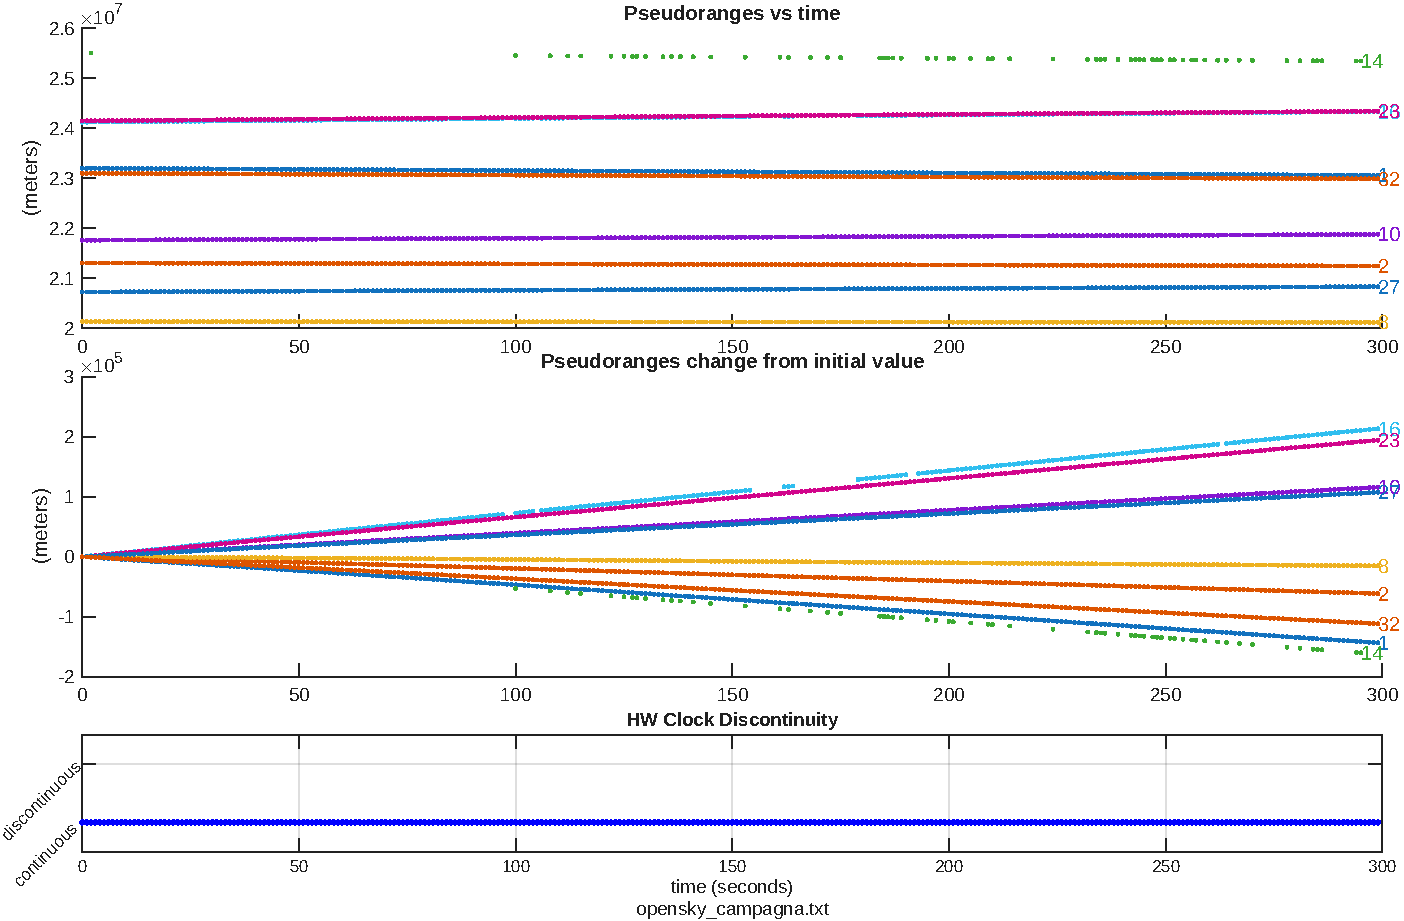
\includegraphics[width=\linewidth]{images/campagna_spoofing_no_delay/Figure_1.pdf}
      %  \caption{Pseudoranges evolution}
       % \label{fig:spoof_far_pr}
    %\end{subfigure}\hfill
    \begin{subfigure}{0.85\columnwidth}
        \centering
        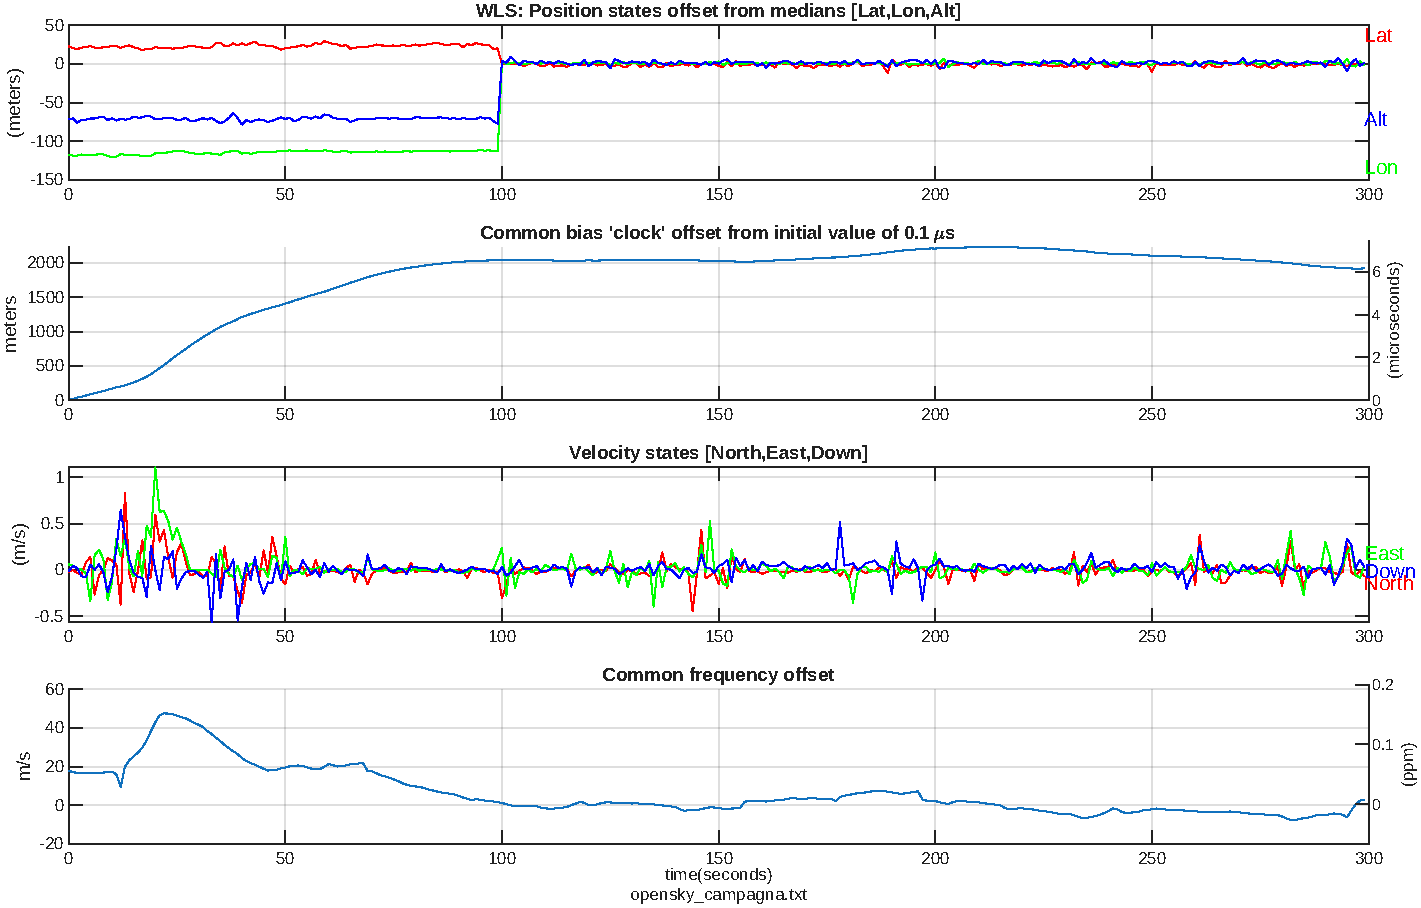
\includegraphics[width=\linewidth]{images/campagna_spoofing_no_delay/Figure_5.pdf}
        \caption{Position states and Clock bias}
        \label{fig:spoof_far_states}
    \end{subfigure}
    \label{fig:spoof_far_results}
\end{figure}

\subsection{Position Spoofing near receiver (with delay)}
In this second scenario, we injected both a false spatial position and a specific \texttt{spoof.delay} of 4 ms: this new addition creates a massive vertical step across all pseudoranges simultaneously. Because satellite signals travel at the speed of light, even a fractional time delay introduced translates into hundreds of kilometers of artificial distance added to every measurement. The WLS solver processes this new measurement and interprets it as a massive receiver clock error. As shown in Figure \ref{fig:spoof_delay_states}, while the spatial coordinates (latitude, longitude, altitude) still snap to the fake location, the clock bias experiences an instant and drastic jump exactly at 100 seconds. This behavior highlights a critical trade-off for an attacker: while introducing a delay might be physically necessary to "capture" the target receiver in a real-world over-the-air attack, it leaves an obvious anomaly in the clock bias domain.

\begin{figure}[htbp]
    \centering
    \begin{subfigure}{0.85\columnwidth}
        \centering
        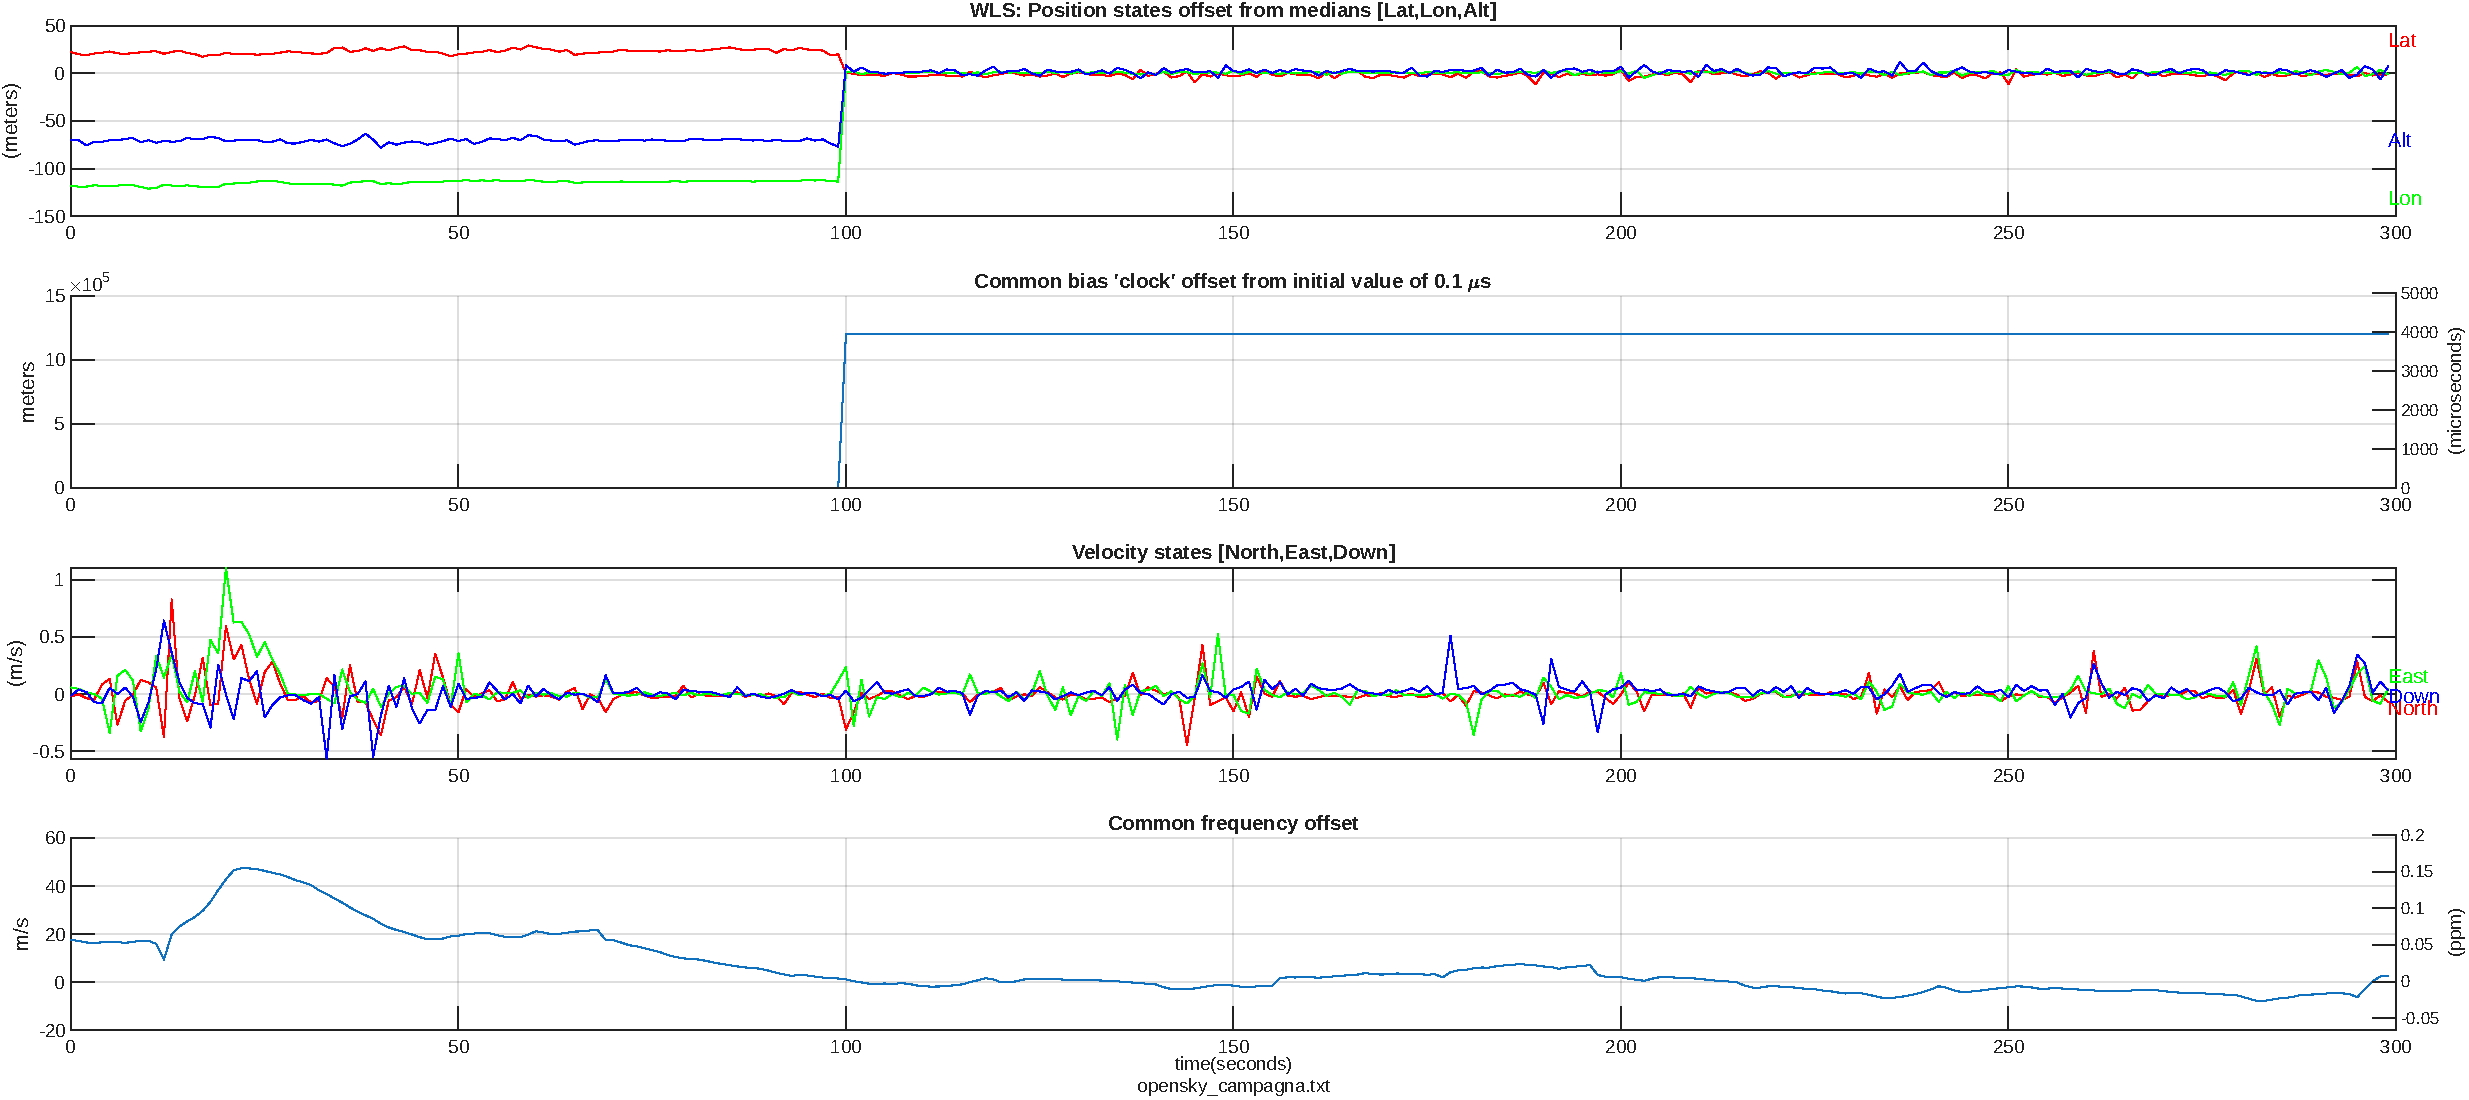
\includegraphics[width=\linewidth]{images/campagna_spoofing_delay/Figure_5.pdf}
        \caption{Position states and Clock bias jump}
        \label{fig:spoof_delay_states}
    \end{subfigure}
    \label{fig:spoof_delay_results}
\end{figure}


\subsection{Position Spoofing far from receiver (with delay)}

Here we executed a harsh spoofing experiment, shifting the target coordinates by approximately 478 km while simultaneously injecting a time delay. This attack represents a worst-case scenario where both the spatial and temporal domains are severely compromised. The "aggressive" spatial translation is visible in the pseudorange rates (Figure \ref{fig:spoof_torino_diff_rate}): in the WLS solution plot the offsets for latitude, longitude and altitude immediately jump on the order of $10^5$ meters. Consequently, the WLS solver is forced to compensate for this artificial propagation delay by forcefully adjusting the receiver's clock. As observed in the previous delayed scenario, the common bias clock violently spikes as shown in Figure \ref{fig:spoof_torino_states_del}. 
\begin{figure}[htbp]
    \centering
    % Prima riga
    \begin{subfigure}{0.48\columnwidth}
        \centering
        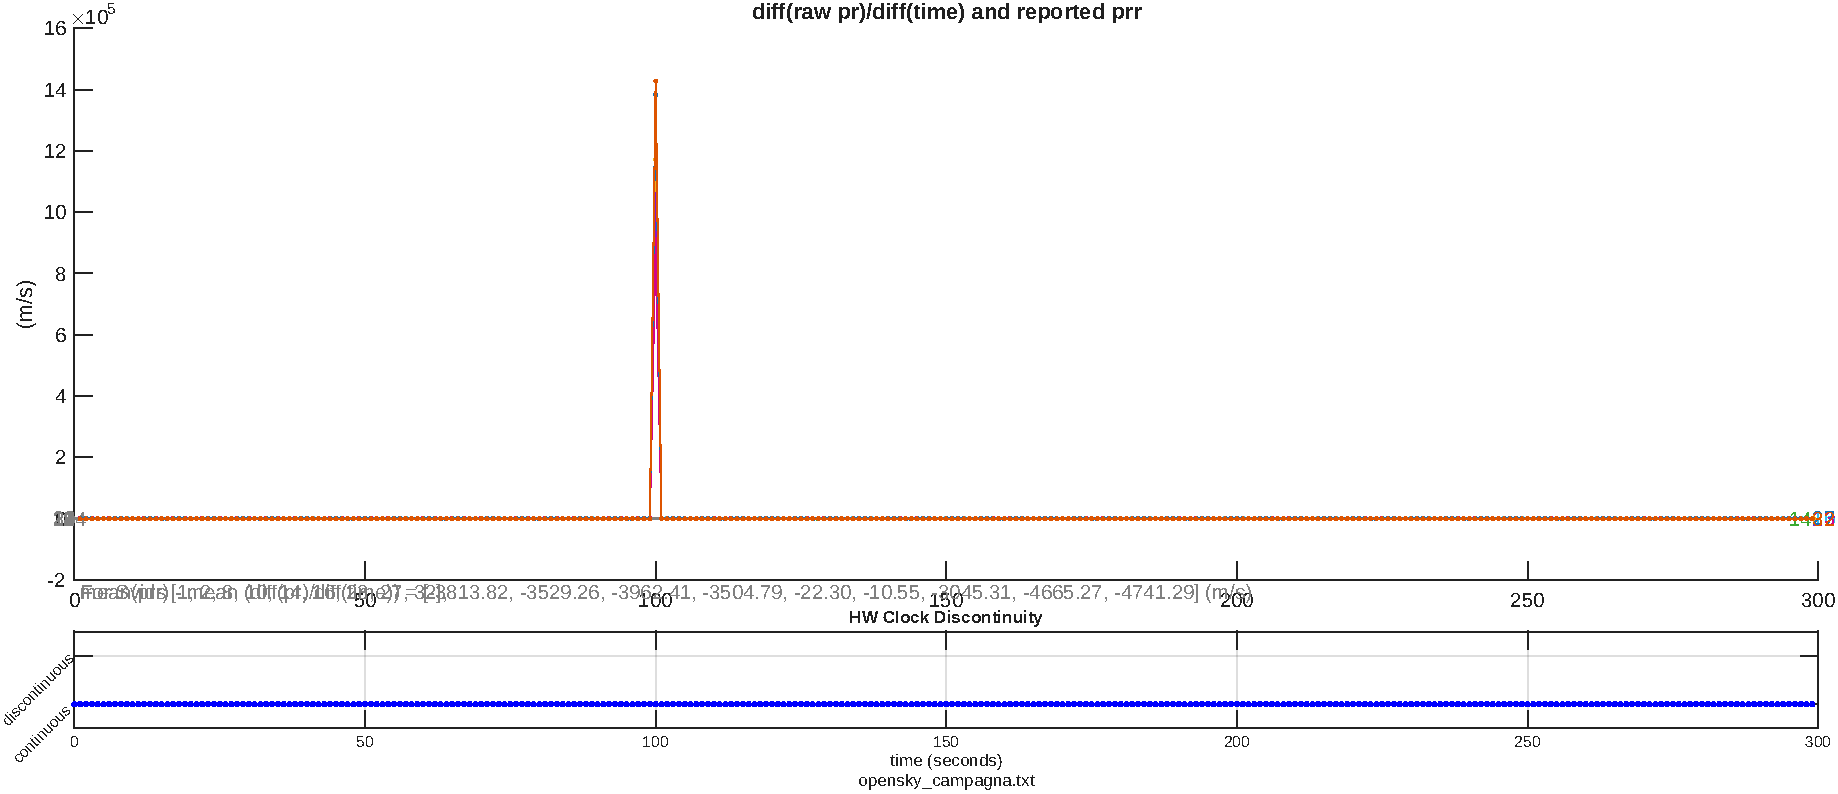
\includegraphics[width=\linewidth]{images/campagna_spoofing_delay_Torino/Figure_2.pdf}
        \caption{Pseudorange rates anomaly}
        \label{fig:spoof_torino_diff_rate}
    \end{subfigure}\hfill
    \begin{subfigure}{0.48\columnwidth}
        \centering
        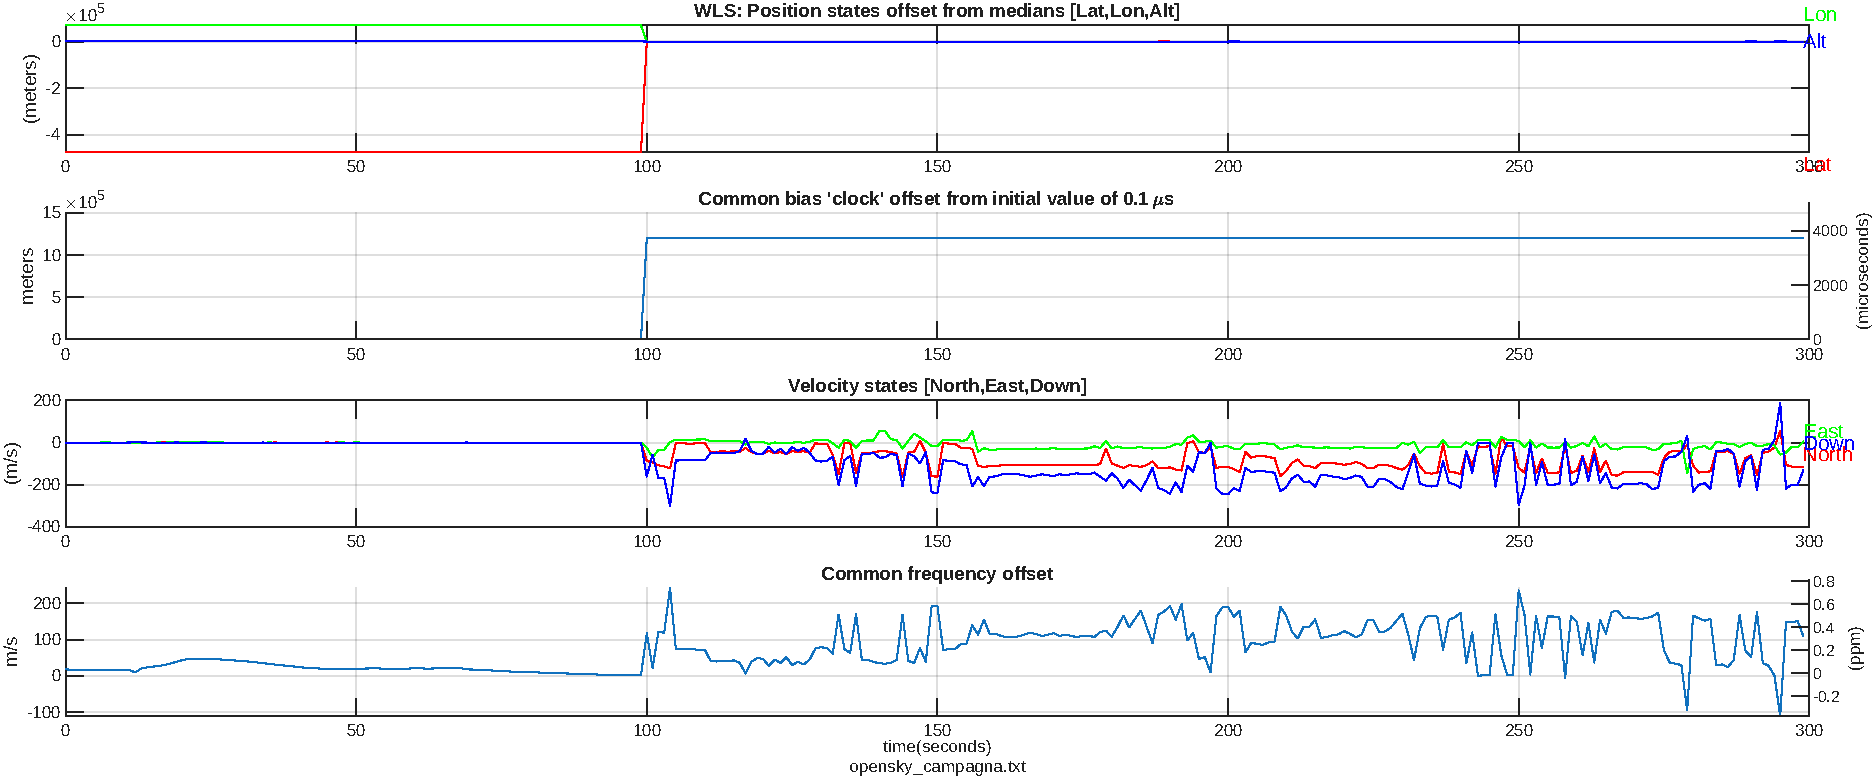
\includegraphics[width=\linewidth]{images/campagna_spoofing_delay_Torino/Figure_5.pdf}
        \caption{Position and Clock bias jump}
        \label{fig:spoof_torino_states_del}
    \end{subfigure}
\end{figure}


\subsection{Position Spoofing far from receiver (without delay)}

Lastly, we simulated another attack by forcing the coordinates similarly to the previous experiment but with the \texttt{spoof.delay} parameter disabled. The magnitude of the spatial jump forces the WLS solver to register again a violent discontinuity in the position states (Figure \ref{fig:spoof_torino_nodelay_states}), with offsets instantly surging by an order of $10^5$ meters and generating a massive change in the pseudorange rates. But the most revealing metric here is the receiver's internal clock: since no artificial time delay was introduced, the common bias clock smoothly follows its natural continuous drift. This physical behavior confirms that the WLS solver interpreted the manipulated measurements strictly as an instantaneous spatial teleportation, compromising the position domain while leaving the temporal synchronization intact.
\begin{figure}[htbp]
    \centering
    \begin{subfigure}{0.85\columnwidth}
        \centering
        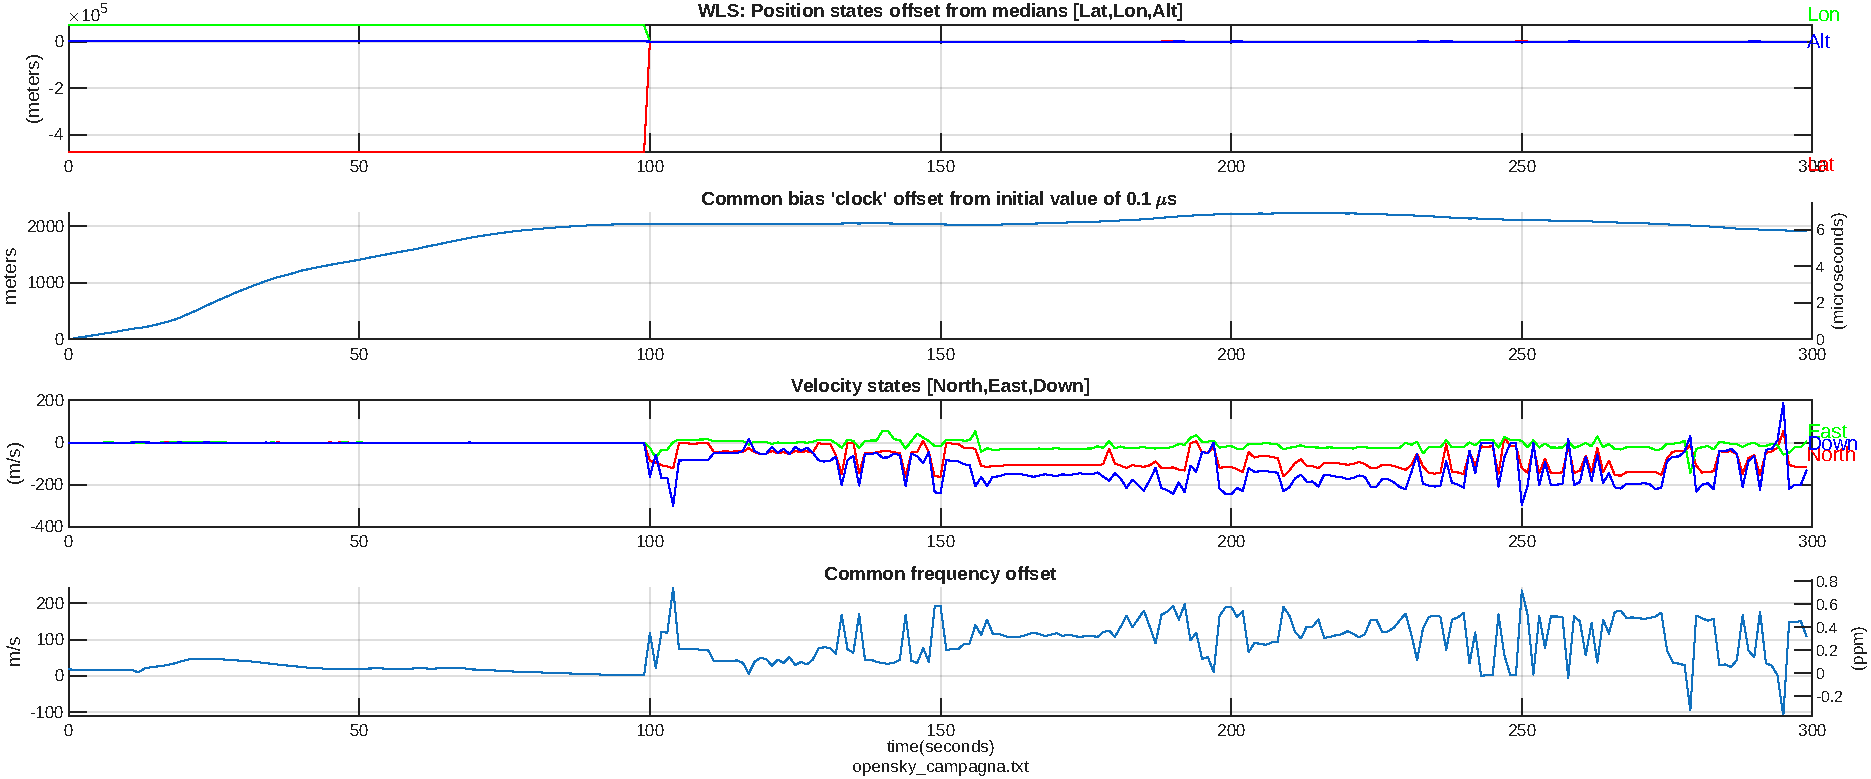
\includegraphics[width=\linewidth]{images/campagna_spoofing_no_delay_Torino/Figure_5.pdf}
        \caption{Position jump of $\times 10^5$ m with continuous clock}
        \label{fig:spoof_torino_nodelay_states}
    \end{subfigure}
    
    % QUESTE RIGHE VUOTE SONO FONDAMENTALI
    \vspace{1cm}
    
    \begin{subfigure}{0.85\columnwidth}
        \centering
        % Ricordati di rinominare il file!
        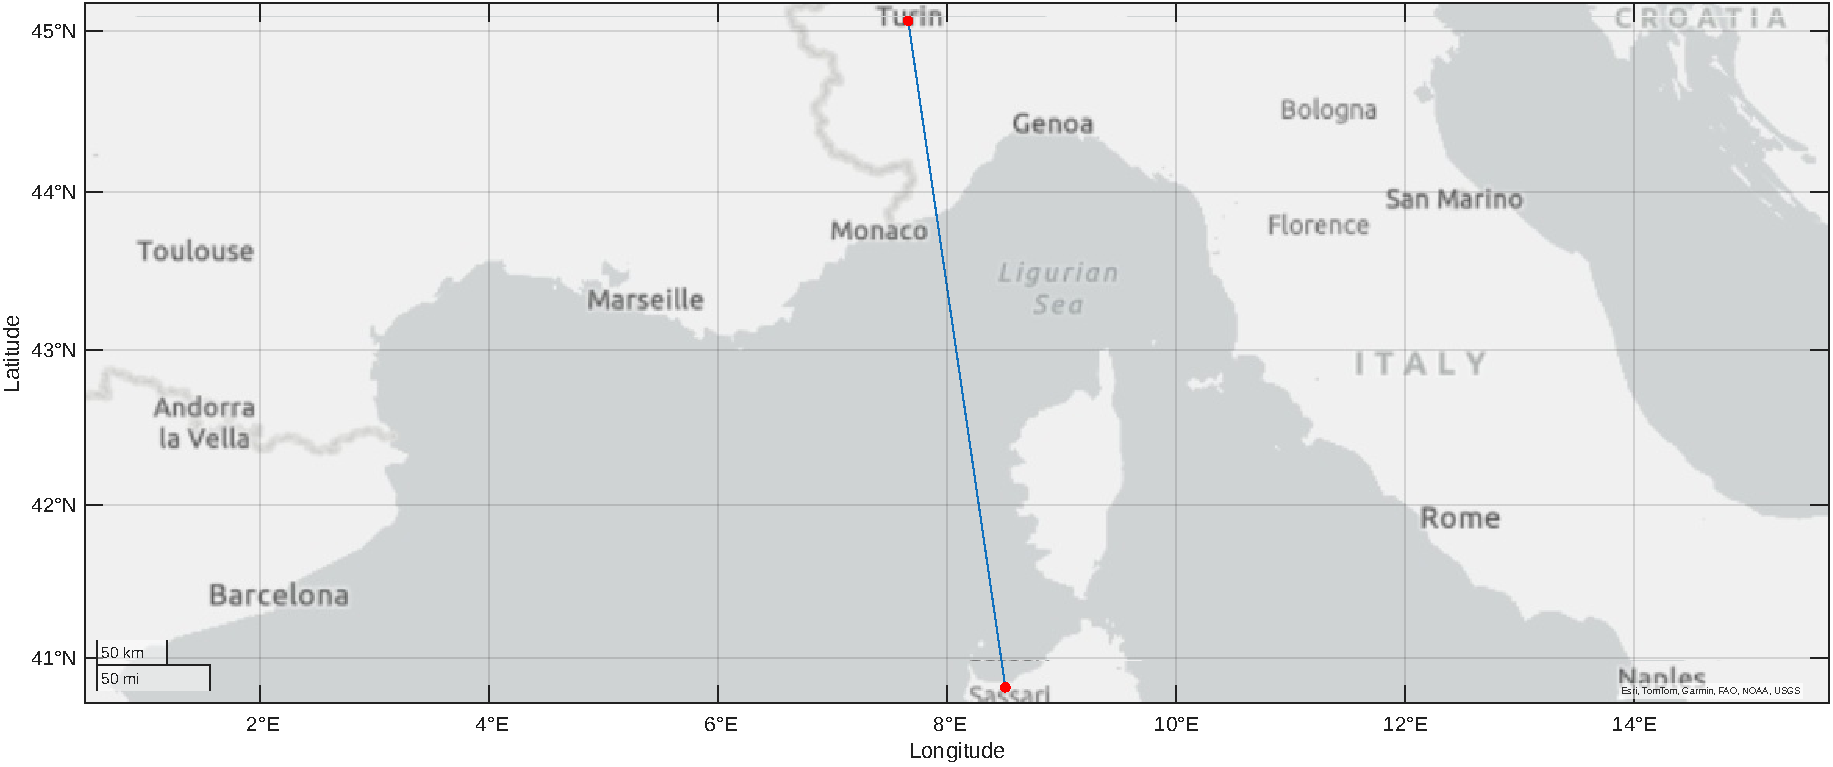
\includegraphics[width=\linewidth]{images/campagna_spoofing_no_delay_Torino/[Optional] Plot Positioning Solution on Map.pdf}
        \caption{Actual location vs spoofed location}
        \label{fig:spoof_torino_nodelay_position}
    \end{subfigure}
    
    \label{fig:spoof_torino_nodelay_results}
\end{figure}

\subsection{Considerations about Spoofing}
The simulation results fully matched our expectations: the pure spatial manipulation successfully altered the physical coordinates in the WLS solver, while the addition of a temporal delay predictably manifested an extreme spike in the hardware clock bias. A reliable spoofing detection strategy could easily track these metrics, flagging physically impossible discontinuities in the pseudorange rates or in the clock bias. From an attacker's perspective, to make the software attack even stealthier, the code could be modified to inject the \texttt{spoof.position} and \texttt{spoof.delay} progressively over time, rather than an instantaneous step: this would keep the horizontal velocity and clock drift within physically plausible limits, with more chances of bypassing basic anomaly detection algorithms.
Furthermore, it is important to note a key characteristic of this purely software-based attack: because the script manipulates the data and does not synthesize a raw signal, the $C/N_0$ plots show absolutely no difference during the attack. In a "real-world" spoofing event, the attacker must also transmit fake signals at a higher power to capture the receiver's tracking loops, generating abrupt variations in the $C/N_0$ levels. Although our data-level injection bypasses these physical-layer checks, monitoring signal strength anomalies remains a primary real-world defense mechanism.
\input{results}
\section{Results and Conclusion}
\label{sec:conclusion}
This study highlighted several vulnerabilities of consumer-grade GNSS receivers. Table \ref{tab:metrics_summary} summarizes the overall performance metrics, confirming the Open Sky scenario as the ideal one for optimal reception. In contrast, introducing electromagnetic shielding and human proximity (during the Aluminum and Body trials) induced drastic attenuation and compromised tracking. The "dynamic" tests also mirrored these challenges: while the moving Bus retained an adequate constellation layout despite reduced power, the Walking path suffered from an "urban canyon" effect, leading to heavy fluctuations and sharp HDOP peaks. We also turned on battery-saving mode multiple times during these experiments, but it showed no predictable (or even significant) impact. Furthermore, our cyber-spoofing simulations proved the ease of manipulating spatial coordinates; although limited by the absence of raw RF transmission, these attacks still left detectable traces. Finally, the collected data confirm that commercial navigation remains highly sensitive to a combination of environmental blockages, multipath interference and software-level attacks.
\\
\begin{table}[htbp]
    \centering
    \caption{Signal Quality and Satellite Geometry}
    \label{tab:metrics_summary}
    \resizebox{\columnwidth}{!}{%
    \begin{tabular}{lcccc}
        \toprule
        \multirow{2}{*}{\textbf{Scenario}} & \multicolumn{2}{c}{\textbf{C/N0 (dB-Hz)}} & \multicolumn{2}{c}{\textbf{HDOP}} \\
        \cmidrule(lr){2-3} \cmidrule(lr){4-5}
        & \textbf{Mean} & \textbf{Std. Dev.} & \textbf{Mean} & \textbf{Std. Dev.} \\
        \midrule
        Open Sky & 35.88 & 5.44 & 1.00 & 0.10 \\
        Outdoor Walking & 27.91 & 5.18 & 1.09 & 0.23 \\
        Outdoor Bus & 27.08 & 3.58 & 1.05 & 0.25 \\
        Body Interference & 32.96 & 6.94 & 1.10 & 0.12 \\
        Aluminum Shielding & 26.67 & 4.37 & 2.08 & 0.65 \\
        \bottomrule
    \end{tabular}%
    }
\end{table}




\bibliographystyle{ACM-Reference-Format}
\bibliography{bib}

% % --- Appendix ---%
\appendix
\input{appendix}

\end{document}


%%% Local Variables:
%%% mode: latex
%%% TeX-master: t
%%% End:
